
\chapter{Modelli lineari: i metodi di soluzione diretti}
\newpage
\minitoc
\newpage
I modelli presentati in questo documento sono gli stessi trattati nel capitolo 1 e 2 del libro ``Computaional Economics. A concise introduction'' di Afonso e Vasconcelos pubblicato nel 2016 dalla casa editrice Routledge.  

\section{\textbf{Il modello domanda e offerta}}\label{sec:domanda-offerta}

\subsection{Il problema economico}

Uno dei problemi più semplici dell'analisi economica consiste nella
determinazione del prezzo e della quantità di equilibrio di un mercato.
Nonostante la sua semplicità, questo problema costituisce un utile punto
di partenza per introdurre alcuni degli strumenti computazionali che
utilizzeremo nel corso.

Consideriamo un mercato nel quale la domanda e l'offerta sono descritte
dalle seguenti funzioni lineari:

\begin{equation}
    Q_d = \bar{Q}_d - aP,
    \label{eq:domanda}
\end{equation}

e

\begin{equation}
    Q_s = \bar{Q}_s + bP,
    \label{eq:offerta}
\end{equation}

dove $Q_d$ rappresenta la quantità domandata, $Q_s$ la quantità
offerta e $P$ il prezzo del bene.

I parametri $\bar{Q}_d$ e $\bar{Q}_s$ rappresentano rispettivamente
le intercette delle funzioni di domanda e di offerta, mentre $a$ e
$b$ ne determinano la sensibilità rispetto al prezzo.

Assumiamo

\begin{equation*}
    a > 0,
    \qquad
    b > 0.
\end{equation*}

La quantità domandata diminuisce quindi all'aumentare del prezzo,
mentre la quantità offerta aumenta.

L'equilibrio del mercato si verifica quando la quantità che i
consumatori desiderano acquistare coincide con quella che i produttori
desiderano vendere. Indicando la quantità di equilibrio con $Q$, la
condizione di equilibrio è pertanto

\begin{equation*}
    Q_d = Q_s = Q.
    \label{eq:equilibrio}
\end{equation*}

Le due variabili endogene del modello sono dunque $Q$ e $P$.
Una volta assegnati i valori dei parametri
$\bar{Q}_d$, $\bar{Q}_s$, $a$ e $b$, il nostro problema consiste nel
determinare il prezzo e la quantità che soddisfano simultaneamente
le equazioni di domanda e di offerta.

In questo semplice modello, possiamo procedere algebricamente sostituendo le equazioni nella condizione di equilibrio:

$$
\underbrace{\bar{Q}_d - aP}_{Q_d}=\underbrace{\bar{Q}_s + bP}_{Q_s}
$$
Solving $P$ we obtain the equilibrium price:
$$
P^*=\frac{\bar Q_d-\bar Q_s}{b-a}.
\label{eq:eqp}
$$
We can use alternatively the demand or the supply function to obtain the equilibrium quantity. Plugging the equilibrium price in the demand equation for example, we get:
$$
Q^*=\bar{Q}_d - aP^*
\label{eq:eqq}
$$

\subsection{Un esempio numerico}

Consideriamo la seguente parametrizzazione:

\begin{equation*}
    \bar{Q}_d = 1000,
    \qquad
    \bar{Q}_s = 250,
    \qquad
    a = 10,
    \qquad
    b = 5.
\end{equation*}

Le funzioni di domanda e di offerta diventano quindi

\begin{equation*}
    Q_d = 1000 - 10P
\end{equation*}

e

\begin{equation*}
    Q_s = 250 + 5P.
\end{equation*}

Per determinare l'equilibrio imponiamo l'uguaglianza tra domanda
e offerta:

\begin{equation*}
    1000 - 10P = 250 + 5P.
\end{equation*}

Riorganizzando i termini otteniamo

\begin{equation*}
    750 = 15P,
\end{equation*}

da cui segue

\begin{equation*}
    P^* = 50.
\end{equation*}

Una volta determinato il prezzo di equilibrio, possiamo sostituirlo
nella funzione di domanda o in quella di offerta per ottenere la quantità di equilibrio. Utilizzando, ad esempio, la funzione di
domanda otteniamo

\begin{equation*}
    Q^* = 1000 - 10(50) = 500.
\end{equation*}

La soluzione del modello è pertanto

\begin{equation*}
    P^* = 50,
    \qquad
    Q^* = 500.
\end{equation*}

Il punto $(P^*,Q^*)$ rappresenta l'equilibrio del mercato.
Graficamente, esso corrisponde al punto di intersezione tra la curva
di domanda e la curva di offerta.

Per prezzi differenti da $P^*$, domanda e offerta non coincidono.
Se il prezzo è inferiore al prezzo di equilibrio, la quantità
domandata è superiore alla quantità offerta e si verifica un
\emph{eccesso di domanda}. Se, al contrario, il prezzo è superiore
al prezzo di equilibrio, la quantità offerta è superiore alla
quantità domandata e si verifica un \emph{eccesso di offerta}.

\subsection{Soluzione al calcolatore}

In questo paragrafo risolveremo il nostro modello utilizzando il calcolatore. La soluzione sarà preceduta da alcune note preliminari sull'utilizzo dei software che riteniamo utili a questo livello.

\subsubsection{Note preliminari}

Per affrontare problemi di calcolo scientifico in economia e finanza sono
disponibili diversi software e linguaggi di programmazione. Tra gli strumenti
maggiormente utilizzati si possono ricordare \textbf{MATLAB},
\textbf{Mathematica} e \textbf{GAMS}, distribuiti con licenza commerciale,
e \textbf{R}, \textbf{Python}, \textbf{Julia} e \textbf{GNU Octave},
disponibili gratuitamente. 

In queste dispense privilegeremo gli strumenti \textbf{gratuiti e open source},
in modo che tutti gli studenti possano utilizzarli liberamente anche al di fuori
delle strutture universitarie. In particolare, faremo riferimento a R, Python,
Julia e GNU Octave. Questi strumenti permettono di affrontare numerosi problemi
di calcolo scientifico, come operazioni con vettori e matrici, soluzione di
sistemi di equazioni, ricerca degli zeri di una funzione, ottimizzazione,
integrazione numerica e simulazione.

Una caratteristica particolarmente utile di questi linguaggi è la possibilità
di lavorare in modo interattivo attraverso un ambiente comunemente indicato
come \textbf{REPL}, acronimo di \emph{Read--Evaluate--Print Loop}. Il
funzionamento di un REPL può essere rappresentato schematicamente come

\[
\text{Read}
\longrightarrow
\text{Evaluate}
\longrightarrow
\text{Print}
\longrightarrow
\text{Loop}
\]

L'ambiente \emph{legge} (\emph{Read}) il comando inserito dall'utente, lo
\emph{valuta ed esegue} (\emph{Evaluate}), ne \emph{mostra} il risultato
(\emph{Print}) e torna quindi in attesa di un nuovo comando (\emph{Loop}).
In questo modo è possibile inserire un'istruzione e osservarne immediatamente
il risultato, senza dover predisporre preventivamente un programma completo.
Questa modalità è particolarmente utile per effettuare calcoli semplici,
sperimentare nuovi comandi e verificare passo dopo passo il funzionamento di
una procedura numerica.

In alternativa, le istruzioni possono essere raccolte in uno
\textbf{script}. Uno script è un file di testo contenente una sequenza di
istruzioni scritte nel linguaggio utilizzato. Il file può essere salvato,
modificato ed eseguito ogni volta che è necessario. Questa modalità è
particolarmente conveniente quando un problema richiede numerosi passaggi,
poiché permette di conservare il codice sviluppato e di eseguire nuovamente
l'intera procedura senza dover reinserire manualmente ogni comando. Inoltre,
l'utilizzo degli script favorisce la \textbf{riproducibilità} dei risultati:
a partire dagli stessi dati e dallo stesso codice è possibile ripetere
l'analisi in un momento successivo o condividerla con altri utenti.

REPL e script non rappresentano due linguaggi differenti, ma due modalità
diverse di utilizzare lo stesso linguaggio. Nel primo caso le istruzioni
vengono generalmente inserite ed eseguite una alla volta; nel secondo vengono
scritte e conservate in un file che può essere successivamente eseguito.

\subsubsection{codice per la soluzione}

La soluzione del nostro modello può essere ottenuta facendo eseguire al software
il codice seguente.

\begin{verbatim}
# definizione dei parametri
a=10
b=5
# definizione delle variabili esogene
Qd_bar=1000
Qs_bar=250
# calcolo del prezzo di equilibrio
Pe=(Qd_bar-Qs_bar)/(a+b)
# calcolo della quantità di equilibrio
Qe=Qd_bar-a*Pe
\end{verbatim}

La sintassi utilizzata in questo codice è accettata, in generale, da diversi
linguaggi per il calcolo scientifico. In particolare, il codice può essere
eseguito, senza modifiche, in R, Python, GNU Octave e Julia. I quattro
linguaggi utilizzano, ad esempio, il simbolo \verb+#+ per indicare l'inizio
di un commento. Tutto ciò che segue questo simbolo sulla stessa
riga non viene interpretato come un'istruzione da eseguire. I commenti
possono quindi essere utilizzati per aggiungere al codice brevi spiegazioni
che ne facilitino la lettura e la comprensione. Ad esempio,
\begin{verbatim}
# definizione dei parametri
a=10
b=5
\end{verbatim}
oppure
\begin{verbatim}
a=10  # parametro della domanda
b=5   # parametro dell'offerta
\end{verbatim}
Esistono tuttavia alcune differenze tra i quattro linguaggi di cui è utile
tenere conto.

La prima riguarda GNU Octave. Se eseguiamo le istruzioni riportate sopra,
Octave visualizza il risultato delle assegnazioni, mentre gli altri linguaggi
non presentano necessariamente lo stesso comportamento. Sebbene questa
caratteristica possa essere utile durante l'esecuzione interattiva, può
produrre una quantità eccessiva di output, soprattutto quando si lavora con
vettori e matrici di grandi dimensioni. In Octave è possibile sopprimere la
visualizzazione del risultato aggiungendo un punto e virgola, \verb+;+,
alla fine dell'istruzione.

Una seconda precisazione riguarda R. In questo linguaggio il simbolo
\verb+=+ può essere utilizzato per effettuare un'assegnazione, ma la
convenzione maggiormente utilizzata è quella di utilizzare l'operatore \verb+<-+. Seguendo tale
convenzione, per adattare il codice precedente allo stile tipico di R è
sufficiente sostituire gli operatori \verb+=+ utilizzati per le assegnazioni
con \verb+<-+. Possiamo scrivere ad esempio:
\begin{verbatim}
a<-10   # parametro della domanda
\end{verbatim}

Infine, per la visualizzazione dei risultati, occorre distinguere tra l'esecuzione interattiva tramite REPL e
l'esecuzione di uno script. Nel REPL, per visualizzare il valore di una
variabile è generalmente sufficiente scriverne il nome e premere Invio. Ad
esempio, digitando
\begin{verbatim}
Pe
\end{verbatim}
viene visualizzato il valore del prezzo di equilibrio. Quando il codice
è contenuto in uno script, invece, è buona pratica utilizzare esplicitamente
le istruzioni messe a disposizione dal linguaggio per visualizzare i risultati
di interesse. La sintassi di tali istruzioni varia da un linguaggio all'altro.

La Tabella~\ref{tab:output_software} riporta, a titolo di esempio, le
istruzioni che possono essere utilizzate per visualizzare il valore della
variabile \verb+Pe+ nei diversi linguaggi considerati.

\begin{table}[ht]
\centering
\caption{Visualizzazione del valore di una variabile nei diversi linguaggi.}
\label{tab:output_software}
\begin{tabular}{lll}
\hline
\textbf{Linguaggio} & \textbf{REPL} & \textbf{Istruzione esplicita} \\
\hline
R         & \verb+Pe+ & \verb+print(Pe)+ \\
Python    & \verb+Pe+ & \verb+print(Pe)+ \\
Julia     & \verb+Pe+ & \verb+println(Pe)+ \\
GNU Octave & \verb+Pe+ & \verb+disp(Pe)+ \\
\hline
\end{tabular}
\end{table}

Si noti che le istruzioni riportate nella terza colonna non sono le uniche
disponibili. I diversi linguaggi offrono infatti ulteriori funzioni per
controllare e formattare l'output.

\subsection{Esperimenti sul modello}

Una volta costruito e risolto il modello, possiamo utilizzarlo per
studiare come cambia l'equilibrio in seguito a una modifica dei
parametri.

Supponiamo, ad esempio, che l'intercetta della funzione di domanda
si riduca da

\begin{equation*}
    \bar{Q}_d = 1000
\end{equation*}

a

\begin{equation*}
    \bar{Q}_d = 750.
\end{equation*}

La funzione di domanda diventa

\begin{equation*}
    Q_d = 750 - 10P.
\end{equation*}

Possiamo quindi risolvere nuovamente il modello, determinare il
nuovo prezzo e la nuova quantità di equilibrio.

Questo semplice esperimento introduce una delle idee fondamentali
dell'economia computazionale. Una volta specificato un modello,
possiamo assegnare valori ai suoi parametri, calcolarne la soluzione
e ripetere il calcolo modificando uno o più parametri per studiare
come cambiano i risultati.

Per poter effettuare efficientemente queste valutazioni, è essenziale utilizzare la modalità scripting mensionata in precedenza.

\subsection{Dall'equilibrio al benessere sociale}

La determinazione di $P^*$ e $Q^*$ non esaurisce 
l'analisi economica che intendiamo effettuare di questo modello. 
Una volta conosciuto l'equilibrio possiamo,
ad esempio, valutare il benessere generato dal mercato attraverso
il surplus dei consumatori e il surplus dei produttori.

Il \emph{surplus del consumatore} misura la differenza tra quanto
i consumatori sarebbero disposti a pagare per le unità acquistate
e quanto effettivamente pagano al prezzo di equilibrio.

Il \emph{surplus del produttore} misura invece la differenza tra
quanto i produttori ricevono dalla vendita delle unità prodotte
e il prezzo minimo al quale sarebbero disposti a offrirle.

Possiamo quindi definire il benessere sociale come

\begin{equation*}
    SW = CS + PS,
    \label{eq:social_welfare}
\end{equation*}

dove $CS$ indica il surplus dei consumatori e $PS$ il surplus
dei produttori.

Nel caso di funzioni lineari, questi surplus possono essere
rappresentati graficamente come aree comprese tra le curve di
domanda e offerta e il prezzo di equilibrio.

Questo passaggio mette in evidenza un aspetto importante
dell'analisi computazionale: la soluzione del modello non
rappresenta necessariamente il risultato finale dell'analisi.
Le variabili di equilibrio ottenute dalla soluzione del modello
possono diventare, a loro volta, input per il calcolo di ulteriori
grandezze di interesse economico.

Il codice relativo a questi calcoli verrà sviluppato dopo che avemo introdotto la forma matriciale del modello.

\subsection{Dal modello economico alla forma matriciale}

Nel semplice esempio precedente il prezzo e la quantità di equilibrio
possono essere determinati facilmente attraverso pochi passaggi
algebrici. Questa strategia diventa tuttavia progressivamente meno
pratica quando aumenta il numero delle equazioni e delle variabili
del modello.

È quindi utile introdurre una rappresentazione più generale del
problema.

Utilizzando la condizione di equilibrio, le equazioni
\eqref{eq:domanda} e \eqref{eq:offerta} possono essere scritte come

\begin{equation*}
    Q = \bar{Q}_d - aP
\end{equation*}

e

\begin{equation*}
    Q = \bar{Q}_s + bP.
\end{equation*}

Portando le variabili endogene a sinistra dell'uguale e i termini noti a destra
otteniamo

\begin{equation*}
    Q + aP = \bar{Q}_d
\end{equation*}

e

\begin{equation*}
    Q - bP = \bar{Q}_s.
\end{equation*}

Le due equazioni possono essere raccolte in un'unica espressione
matriciale:

\begin{equation*}
    \begin{pmatrix}
        1 & a \\
        1 & -b
    \end{pmatrix}
    \begin{pmatrix}
        Q \\
        P
    \end{pmatrix}
    =
    \begin{pmatrix}
        \bar{Q}_d \\
        \bar{Q}_s
    \end{pmatrix}.
    \label{eq:domanda_offerta_matrice}
\end{equation*}

Definiamo ora

\begin{equation*}
    A =
    \begin{pmatrix}
        1 & a \\
        1 & -b
    \end{pmatrix},
    \qquad
    x =
    \begin{pmatrix}
        Q \\
        P
    \end{pmatrix},
    \qquad
    d =
    \begin{pmatrix}
        \bar{Q}_d \\
        \bar{Q}_s
    \end{pmatrix}.
\end{equation*}

Il modello può quindi essere scritto nella forma compatta

\begin{equation}
    Ax=d.
    \label{eq:sistema_lineare_generale}
\end{equation}

La rappresentazione matriciale non modifica il contenuto economico
del modello. Il prodotto matrice-vettore $Ax$ (che verrà illustrato nel prosieguo) ricostruisce infatti,
riga per riga, le equazioni originarie.

Il vantaggio della rappresentazione \eqref{eq:sistema_lineare_generale}
è che permette di riconoscere nel nostro semplice modello di domanda
e offerta un problema matematico molto più generale: la soluzione
di un sistema di equazioni lineari.

\subsection{Il problema computazionale}

Il modello di domanda e offerta ci ha quindi condotto a un problema
che incontreremo ripetutamente nel corso.

Data una matrice $A$ e un vettore $d$, vogliamo determinare il
vettore $x$ tale che

\begin{equation*}
    Ax=d.
\end{equation*}

Nel nostro esempio, $x$ contiene soltanto due elementi, il prezzo
e la quantità di equilibrio. Nei modelli più complessi, tuttavia,
$x$ può contenere decine, centinaia o anche migliaia di incognite.

Diventa allora necessario disporre di procedure sistematiche ed
efficienti per risolvere il sistema.

Prima di studiare queste procedure è opportuno richiamare alcuni
concetti dell'algebra matriciale che saranno utilizzati nella
costruzione degli algoritmi numerici. Essi costituiscono l'oggetto
del prossimo paragrafo.

\section{\textit{\textbf{Strumenti di matematica}}: le matrici}


Nel paragrafo precedente abbiamo visto che un semplice modello di
domanda e offerta può essere rappresentato mediante un sistema di
equazioni lineari della forma

\begin{equation*}
    Ax=b.
    \label{eq:sistema_lineare}
\end{equation*}

Questa rappresentazione sarà utilizzata ripetutamente nel corso.
Prima di affrontare i metodi numerici che consentono di calcolare
la soluzione di un sistema lineare, è quindi utile richiamare alcuni
concetti fondamentali dell'algebra matriciale.

L'obiettivo di questo paragrafo non è fornire una trattazione completa
dell'algebra lineare, ma introdurre gli strumenti che saranno
necessari per comprendere i metodi numerici presentati nei capitoli
successivi.


\subsection{Vettori e matrici}

Un \emph{vettore} è un insieme ordinato di numeri. 
Un vettore composto da $n$ elementi può essere rappresentato come

\begin{equation*}
\mathbf{x} =
\begin{pmatrix}
x_1 \\
x_2 \\
\vdots \\
x_n
\end{pmatrix}.
\end{equation*}

Gli elementi $x_1,x_2,\ldots,x_n$ sono detti \emph{componenti}
del vettore. Se le componenti sono numeri reali, un vettore con
$n$ componenti appartiene allo spazio $\mathbb{R}^n$, e scriviamo

\begin{equation*}
\mathbf{x} \in \mathbb{R}^n.
\end{equation*}

Per convenzione, salvo diversa indicazione, considereremo i vettori
come \emph{vettori colonna}. Un vettore può tuttavia essere
rappresentato anche come vettore riga. Il vettore riga associato a
$\mathbf{x}$ si ottiene mediante l'operazione di trasposizione:

\begin{equation*}
\mathbf{x}^T =
\begin{pmatrix}
x_1 & x_2 & \cdots & x_n
\end{pmatrix}.
\end{equation*}

Un vettore può essere visto come un caso particolare di matrice:
un vettore colonna con $n$ componenti è una matrice di dimensione
$n\times 1$, mentre un vettore riga è una matrice di dimensione
$1\times n$.

Una matrice è un insieme di numeri organizzati in righe e colonne.
Una matrice con $m$ righe e $n$ colonne può essere rappresentata come
\begin{equation*}
A =
\begin{pmatrix}
a_{11} & a_{12} & \cdots & a_{1n} \\
a_{21} & a_{22} & \cdots & a_{2n} \\
\vdots & \vdots & \ddots & \vdots \\
a_{m1} & a_{m2} & \cdots & a_{mn}
\end{pmatrix}.
\end{equation*}
L'elemento $a_{ij}$ indica l'elemento che si trova nella riga $i$
e nella colonna $j$.

Quando il numero delle righe coincide con quello delle colonne,
la matrice viene detta \emph{quadrata}. 
Una matrice quadrata $A$ di dimensione $n$ con elementi reali
appartiene allo spazio $\mathbb{R}^{n\times n}$, e scriviamo
\begin{equation*}
A \in \mathbb{R}^{n\times n}.
\end{equation*}

Alcune particolari matrici quadrate avranno un ruolo importante
nei metodi numerici che studieremo.


\subsubsection{Matrice diagonale}

Una matrice è detta \emph{diagonale} quando tutti gli elementi
al di fuori della diagonale principale sono nulli:

\begin{equation*}
D =
\begin{pmatrix}
d_{11} & 0      & \cdots & 0 \\
0      & d_{22} & \cdots & 0 \\
\vdots & \vdots & \ddots & \vdots \\
0      & 0      & \cdots & d_{nn}
\end{pmatrix}.
\end{equation*}


\subsubsection{Matrici triangolari}

Una matrice è \emph{triangolare superiore} quando tutti gli
elementi al di sotto della diagonale principale sono nulli:

\begin{equation*}
U =
\begin{pmatrix}
u_{11} & u_{12} & \cdots & u_{1n} \\
0      & u_{22} & \cdots & u_{2n} \\
\vdots & \ddots & \ddots & \vdots \\
0      & \cdots & 0      & u_{nn}
\end{pmatrix}.
\end{equation*}

Analogamente, una matrice è \emph{triangolare inferiore} quando
sono nulli tutti gli elementi al di sopra della diagonale:

\begin{equation*}
L =
\begin{pmatrix}
l_{11} & 0      & \cdots & 0 \\
l_{21} & l_{22} & \cdots & 0 \\
\vdots & \vdots & \ddots & \vdots \\
l_{n1} & l_{n2} & \cdots & l_{nn}
\end{pmatrix}.
\end{equation*}

Queste matrici avranno particolare importanza quando introdurremo
i metodi numerici per la soluzione dei sistemi lineari.


\subsubsection{Matrice identità}

Un caso particolare di matrice diagonale è la matrice identità,

\begin{equation*}
I =
\begin{pmatrix}
1 & 0 & \cdots & 0 \\
0 & 1 & \cdots & 0 \\
\vdots & \vdots & \ddots & \vdots \\
0 & 0 & \cdots & 1
\end{pmatrix}.
\end{equation*}

La matrice identità svolge nel prodotto tra matrici un ruolo
analogo a quello svolto dal numero $1$ nella moltiplicazione
tra numeri. Per una matrice $A$ di dimensioni compatibili vale

\begin{equation*}
AI=IA=A.
\end{equation*}


\paragraph{Matrice trasposta e matrici simmetriche}

La \emph{trasposta} di una matrice $A$ si ottiene scambiando
le righe con le colonne. Essa viene indicata con $A^T$. Espresso in modo più diretto, la prima riga di $A$ diventa la prima colonna di $A^T$, la seconda riga di $A$ diventa la seconda colonna di $A^T$ e così via. 

Se, ad esempio,
\begin{equation*}
A =
\begin{pmatrix}
a & b \\
c & d
\end{pmatrix},
\end{equation*}
allora
\begin{equation*}
A^T =
\begin{pmatrix}
a & c \\
b & d
\end{pmatrix}.
\end{equation*}

La trasposta di una matrice triangolare superiore è quindi una
matrice triangolare inferiore, e viceversa.

Una matrice quadrata è detta \emph{simmetrica} quando coincide
con la propria trasposta:

\begin{equation*}
A=A^T.
\end{equation*}

Equivalentemente, in una matrice simmetrica vale

\begin{equation*}
a_{ij}=a_{ji}.
\end{equation*}

La simmetria sarà una proprietà importante perché alcune tecniche
numeriche possono essere utilizzate in modo particolarmente
efficiente quando la matrice del sistema possiede questa
caratteristica.


\subsection{Operazioni tra matrici}

Per utilizzare la rappresentazione matriciale dei modelli è
necessario conoscere alcune operazioni fondamentali.


\subsubsection{Somma}

Due matrici $A$ e $B$ con le stesse dimensioni possono essere
sommate elemento per elemento. Se

\begin{equation*}
C=A+B,
\end{equation*}

allora

\begin{equation*}
c_{ij}=a_{ij}+b_{ij}.
\end{equation*}


\subsubsection{Moltiplicazione per uno scalare}

Se $d$ è un numero reale e $A$ una matrice, il prodotto

\begin{equation*}
C=dA
\end{equation*}

si ottiene moltiplicando ogni elemento di $A$ per $d$:

\begin{equation*}
c_{ij}=d\,a_{ij}.
\end{equation*}


\subsubsection{Prodotto tra matrici}

Il prodotto tra matrici richiede maggiore attenzione. Date due
matrici $A$ e $B$, il prodotto

\begin{equation*}
C=AB
\end{equation*}

è definito se il numero di colonne di $A$ coincide con il numero
di righe di $B$.

Ogni elemento della matrice risultante viene ottenuto moltiplicando
gli elementi della corrispondente riga di $A$ per quelli della
corrispondente colonna di $B$ e sommando i prodotti. Possiamo formalizzare quanto appena detto come segue:

\begin{equation*}
c_{ij}=\sum_z a_{iz}b_{zj}.
\label{eq:prodotto_matrici}
\end{equation*}

Se $A$ ha dimensione $m\times n$ e $B$ ha dimensione $n\times p$,
la matrice risultante $C=AB$ avrà dimensione $m\times p$.

È importante osservare che, in generale,

\begin{equation*}
AB \neq BA.
\end{equation*}

Il prodotto tra matrici non gode quindi della proprietà commutativa.

Questa regola di moltiplicazione spiega perché il sistema

\begin{equation*}
Ax=b
\end{equation*}

rappresenta simultaneamente tutte le equazioni di un modello.
Ogni riga della matrice $A$, moltiplicata per il vettore $x$,
genera infatti una delle equazioni del sistema.


\subsection{Traccia e determinante}

A una matrice quadrata possono essere associate alcune grandezze
scalari. Tra queste consideriamo la traccia e il determinante.


\subsubsection{Traccia}

La \emph{traccia} di una matrice quadrata è la somma degli elementi
della diagonale principale:

\begin{equation*}
\operatorname{tr}(A)
=
\sum_{i=1}^{n}a_{ii}.
\end{equation*}

Ad esempio, se

\begin{equation*}
A=
\begin{pmatrix}
2 & 3 \\
4 & 5
\end{pmatrix},
\end{equation*}

allora

\begin{equation*}
\operatorname{tr}(A)=2+5=7.
\end{equation*}


\subsubsection{Determinante}

Il \emph{determinante} associa a una matrice quadrata $A$ un
numero reale, indicato con

\begin{equation*}
\det(A).
\end{equation*}

Il determinante avrà un ruolo importante nello studio dei sistemi
lineari perché consente, tra le altre cose, di stabilire se una
matrice quadrata è invertibile.


\paragraph{Calcolo del determinante}

Per una matrice generale di dimensione $n\times n$, il determinante
può essere calcolato mediante lo sviluppo di Laplace.

Scegliendo una qualsiasi riga $i$,

\begin{equation*}
\det(A)
=
\sum_{j=1}^{n}
a_{ij}(-1)^{i+j}\det(A_{ij}),
\label{eq:laplace_riga}
\end{equation*}

dove $A_{ij}$ è la matrice ottenuta eliminando da $A$ la riga $i$
e la colonna $j$.

In modo equivalente, scegliendo una colonna $j$,

\begin{equation*}
\det(A)
=
\sum_{i=1}^{n}
a_{ij}(-1)^{i+j}\det(A_{ij}).
\label{eq:laplace_colonna}
\end{equation*}

Il risultato non dipende dalla riga o dalla colonna scelta per
effettuare lo sviluppo.

La natura ricorsiva di questa procedura rende tuttavia il calcolo
del determinante progressivamente più laborioso all'aumentare
della dimensione della matrice. Questo aspetto sarà importante
quando passeremo dalla soluzione algebrica di piccoli sistemi
alla loro soluzione numerica.


\paragraph{Il caso delle matrici triangolari}

Il calcolo del determinante è particolarmente semplice nel caso
delle matrici diagonali e triangolari.

Se $A$ è triangolare o diagonale, vale infatti

\begin{equation*}
\det(A)=\prod_{i=1}^{n}a_{ii}.
\label{eq:det_triangolare}
\end{equation*}

Il determinante è quindi semplicemente il prodotto degli elementi
della diagonale principale.



\subsubsection{Matrici singolari e non singolari}

Una matrice quadrata $A$ è detta \emph{non singolare} quando

\begin{equation*}
\det(A)\neq 0.
\end{equation*}

Se invece

\begin{equation*}
\det(A)=0,
\end{equation*}

la matrice è detta \emph{singolare}.

Questa distinzione è fondamentale per il problema che stiamo
studiando. Una matrice $A$ possiede infatti una matrice inversa
se e solo se è non singolare.

Ricordando quanto detto al paragrafo precedente, possiamo dire che una matrice triangolare è non singolare se tutti gli elementi della sua diagonale sono diversi da zero.

\subsection{La matrice inversa}

Se una matrice è non singolare, allora esiste la sua inversa.

L'inversa di una matrice quadrata $A$, indicata con $A^{-1}$,
è definita come la matrice che soddisfa

\begin{equation*}
A^{-1}A=I.
\end{equation*}

dove $I$ è la matrice identità definita in precedenza.

Vale inoltre

\begin{equation*}
AA^{-1}=I.
\end{equation*}

L'analogia con i numeri reali è immediata. Se $a\neq0$, il suo
inverso $a^{-1}=1/a$ soddisfa

\begin{equation*}
a^{-1}a=1.
\end{equation*}

Come ricordato in precedenza, nel caso delle matrici, il ruolo del numero $1$ è svolto dalla
matrice identità $I$.


\subsection{Soluzione di un sistema lineare}

\subsubsection{Approccio teorico}
Riportiamo di seguito due metodi classici per la soluzione di sistemi di equazioni lineari: il \textbf{metodo dell'inversa} e la \textbf{regola di Cramer}. Questi metodi sono utili per comprendere le proprietà algebriche dei sistemi lineari e possono essere applicati agevolmente a sistemi di piccole dimensioni. Tuttavia, dal punto di vista computazionale, diventano inefficienti all'aumentare della dimensione del sistema e non rappresentano, in generale, i metodi utilizzati per la soluzione numerica di sistemi di grandi dimensioni. Successivamente introdurremo pertanto algoritmi numericamente più efficienti, maggiormente utilizzati nelle applicazioni pratiche.

\paragraph{Soluzione mediante la matrice inversa}

Torniamo ora al problema dal quale siamo partiti:

\begin{equation*}
Ax=b.
\end{equation*}

Se $A$ è non singolare, esiste $A^{-1}$. Possiamo quindi
premoltiplicare entrambi i membri dell'equazione per $A^{-1}$:

\begin{equation*}
A^{-1}Ax=A^{-1}b.
\end{equation*}

Poiché

\begin{equation*}
A^{-1}A=I,
\end{equation*}

otteniamo

\begin{equation*}
Ix=A^{-1}b.
\end{equation*}

Infine, dato che $Ix=x$,

\begin{equation*}
x=A^{-1}b.
\label{eq:soluzione_inversa}
\end{equation*}

Abbiamo quindi ottenuto una formula che, almeno dal punto di vista
algebrico, permette di risolvere il sistema lineare.


\paragraph{Dal risultato al problema computazionale}

La relazione

\begin{equation*}
x=A^{-1}b
\end{equation*}

fornisce una soluzione elegante del problema dal punto di vista
matematico. Potrebbe quindi sembrare che il problema posto alla
fine del capitolo precedente sia già risolto: basta calcolare
l'inversa di $A$ e moltiplicarla per $b$.

Dal punto di vista computazionale, tuttavia, rimane una questione
fondamentale:

Il calcolo della matrice inversa è agevole dal punto di vista computazionale?

Purtroppo, il numero di operazioni che il calcolatore deve effettuare, cresce molto rapidamente all'aumentare della dimensione del sistema.

Dunque, ancorché calcolare l'inversa sia possibile per piccoli sistemi, occorre identificare strategie alternative. 

%Per sistemi di piccole dimensioni la distinzione può sembrare poco importante. Quando il numero delle equazioni cresce, invece, il numero di operazioni richieste e il modo in cui esse vengono organizzate diventano elementi centrali.

La formula $x=A^{-1}b$ deve quindi essere interpretata innanzitutto
come una caratterizzazione matematica della soluzione. Non implica
necessariamente che il calcolo esplicito dell'inversa sia il modo
più conveniente per ottenere numericamente $x$.

Questo ci conduce direttamente al problema affrontato nel prossimo
capitolo: individuare procedure più adatte per risolvere un sistema
lineare senza dover necessariamente calcolare esplicitamente
$A^{-1}$.

\paragraph{Soluzione mediante regola di Cramer}
\label{sec:eliminazione-gaussiana}

Nella sezione precedente abbiamo visto che, se la matrice $A$ è
non singolare, il sistema lineare

\begin{equation*}
    Ax=b
\end{equation*}

ammette una soluzione unica, che può essere espressa formalmente come

\begin{equation*}
    x=A^{-1}b.
\end{equation*}

Questa espressione caratterizza la soluzione dal punto di vista
matematico, ma non implica che il calcolo esplicito della matrice
inversa rappresenti il modo più conveniente per determinarla.

Un'altra possibilità, nota dall'algebra lineare, è rappresentata
dalla regola di Cramer. Per un sistema di $n$ equazioni in $n$
incognite, ciascun elemento della soluzione può essere scritto come

\begin{equation*}
    x_i =
    \frac{\det(A_i)}{\det(A)},
    \qquad i=1,\ldots,n,
    \label{eq:cramer}
\end{equation*}

dove $A_i$ è la matrice ottenuta sostituendo la $i$-esima colonna
di $A$ con il vettore $b$.

Anche questa formula fornisce una caratterizzazione esatta della
soluzione. Tuttavia, il suo utilizzo richiede il calcolo di numerosi
determinanti. Il costo computazionale cresce quindi molto rapidamente
all'aumentare della dimensione del sistema. La regola di Cramer è
utile per comprendere alcune proprietà teoriche dei sistemi lineari,
ma non costituisce un metodo efficiente per la soluzione numerica di
sistemi di grandi dimensioni.

Occorre quindi cercare una procedura che permetta di ottenere la
soluzione senza calcolare esplicitamente l'inversa di $A$ e senza
dover calcolare un determinante per ogni incognita.

\subsubsection{Approccio operativo: l'eliminazione gaussiana}

Una delle procedure fondamentali per raggiungere questo obiettivo è
l'\emph{eliminazione gaussiana}.


\subsubsection{L'idea dell'eliminazione gaussiana}

L'idea alla base dell'eliminazione gaussiana consiste nel trasformare
il sistema originario in un sistema equivalente, ma più semplice da
risolvere.

In particolare, si cerca di trasformare la matrice del sistema in una
matrice triangolare. Come vedremo, un sistema caratterizzato da una
matrice triangolare può essere risolto in modo particolarmente
semplice, procedendo sequenzialmente da un'equazione all'altra.

Per descrivere contemporaneamente i coefficienti del sistema e i
termini noti, è conveniente costruire la \emph{matrice aumentata}

\begin{equation*}
    C = [A \mid b].
    \label{eq:matrice-aumentata}
\end{equation*}

L'eliminazione gaussiana modifica progressivamente questa matrice
attraverso operazioni che non modificano la soluzione del sistema.
In questo modo otteniamo una successione di sistemi equivalenti,
fino a raggiungere una forma che può essere risolta facilmente.


\paragraph{Operazioni elementari sulle righe}
Le trasformazioni utilizzate nell'eliminazione gaussiana sono
costituite da tre operazioni elementari sulle righe della matrice
aumentata:

\begin{enumerate}
    \item scambiare la posizione di due righe;
    
    \item moltiplicare tutti gli elementi di una riga per uno
    scalare non nullo;
    
    \item sostituire una riga con la somma della stessa riga e
    di un multiplo di un'altra riga.
\end{enumerate}

Queste operazioni trasformano il sistema in un sistema equivalente:
cambiano cioè la forma nella quale le equazioni sono rappresentate,
ma non l'insieme delle loro soluzioni.

La terza operazione è particolarmente importante. Scegliendo
opportunamente il coefficiente con il quale moltiplicare una riga,
possiamo infatti annullare uno degli elementi della matrice.
Ripetendo questa operazione possiamo progressivamente ottenere una
matrice triangolare.

Procediamo di seguito con l'applicazione del metodo di Gauss al modello di domanda e offerta. Nei prossimi modelli introdurremo altri metodi operativi per la soluzione dei sistemi di equazioni lineari, particolarmente utili quando la dimensione del sistema aumenta o quando occorre risolvere più volte sistemi caratterizzati dalla stessa matrice dei coefficienti. In particolare, considereremo i metodi basati sulla \textbf{fattorizzazione della matrice dei coefficienti}, come la fattorizzazione LU e la fattorizzazione di Cholesky.

\section{Soluzione del modello di domanda e offerta}
\subsection{L'equilibrio}
Riprendiamo il modello di domanda e offerta introdotto nella
Sezione~\ref{sec:domanda-offerta}. Il sistema è

\begin{equation*}
    Ax=b,
\end{equation*}

con

\begin{equation*}
    A=
    \begin{pmatrix}
        1 & a\\
        1 & -b
    \end{pmatrix},
    \qquad
    x=
    \begin{pmatrix}
        Q\\
        P
    \end{pmatrix},
    \qquad
    b=
    \begin{pmatrix}
        \bar Q_d\\
        \bar Q_s
    \end{pmatrix}.
\end{equation*}

Utilizzando i valori

\begin{equation*}
    \bar Q_d=1000,
    \qquad
    \bar Q_s=250,
    \qquad
    a=10,
    \qquad
    b=5,
\end{equation*}

otteniamo

\begin{equation*}
    \begin{pmatrix}
        1 & 10\\
        1 & -5
    \end{pmatrix}
    \begin{pmatrix}
        Q\\
        P
    \end{pmatrix}
    =
    \begin{pmatrix}
        1000\\
        250
    \end{pmatrix}.
    \label{eq:sistema-domanda-offerta-gauss}
\end{equation*}

La corrispondente matrice aumentata è

\begin{equation*}
    C=[A\mid b]
    =
    \left(
    \begin{array}{cc|c}
        1 & 10 & 1000\\
        1 & -5 & 250
    \end{array}
    \right).
    \label{eq:matrice-aumentata-domanda-offerta}
\end{equation*}

Il nostro obiettivo è trasformare questa matrice in modo da
eliminare una delle due incognite da una delle equazioni.


\subsubsection{Una prima trasformazione}

Una prima possibilità consiste nel sostituire la prima riga con la
somma della prima riga e della seconda riga moltiplicata per 2. Indicando le
righe con $R_1$ e $R_2$, l'operazione può essere scritta come

\begin{equation*}
    R_1 \leftarrow R_1+2R_2.
\end{equation*}

Applicando l'operazione alla matrice aumentata otteniamo

\begin{equation*}
    \left(
    \begin{array}{cc|c}
        1 & 10 & 1000\\
        1 & -5 & 250
    \end{array}
    \right)
    \longrightarrow
    \left(
    \begin{array}{cc|c}
        3 & 0 & 1500\\
        1 & -5 & 250
    \end{array}
    \right).
\end{equation*}

La prima equazione del nuovo sistema è quindi

\begin{equation*}
    3Q=1500,
\end{equation*}

da cui otteniamo immediatamente

\begin{equation*}
    Q=500.
\end{equation*}

Conosciuto $Q$, possiamo utilizzare la seconda equazione,

\begin{equation*}
    Q-5P=250,
\end{equation*}

e sostituire il valore appena calcolato:

\begin{equation*}
    500-5P=250.
\end{equation*}

Da cui

\begin{equation*}
    P=50.
\end{equation*}

Otteniamo pertanto nuovamente la soluzione

\begin{equation*}
    x^*=
    \begin{pmatrix}
        500\\
        50
    \end{pmatrix}.
\end{equation*}


\subsubsection{Una seconda trasformazione}

La sequenza di operazioni utilizzata per risolvere un sistema non è
necessariamente unica. Nel nostro semplice esempio possiamo, ad
esempio, scegliere di sostituire la prima riga con la differenza tra
la prima e la seconda riga:

\begin{equation*}
    R_1 \leftarrow R_1-R_2.
\end{equation*}

Otteniamo

\begin{equation*}
    \left(
    \begin{array}{cc|c}
        1 & 10 & 1000\\
        1 & -5 & 250
    \end{array}
    \right)
    \longrightarrow
    \left(
    \begin{array}{cc|c}
        0 & 15 & 750\\
        1 & -5 & 250
    \end{array}
    \right).
\end{equation*}

La prima equazione è ora

\begin{equation*}
    15P=750,
\end{equation*}

da cui

\begin{equation*}
    P=50.
\end{equation*}

Sostituendo questo valore nella seconda equazione,

\begin{equation*}
    Q-5P=250,
\end{equation*}

otteniamo

\begin{equation*}
    Q-5(50)=250,
\end{equation*}

e quindi

\begin{equation*}
    Q=500.
\end{equation*}

Anche questa sequenza di trasformazioni conduce dunque alla stessa
soluzione:

\begin{equation*}
    Q^*=500,
    \qquad
    P^*=50.
\end{equation*}


\subsubsection{Dall'esempio all'algoritmo}

Il sistema di domanda e offerta contiene soltanto due equazioni e
una singola operazione di eliminazione è sufficiente per renderlo
immediatamente risolvibile. Tuttavia, la stessa idea può essere
applicata a sistemi con un numero maggiore di equazioni.

In termini generali, l'eliminazione gaussiana utilizza le operazioni
elementari sulle righe per eliminare progressivamente le incognite
dalle diverse equazioni. L'obiettivo è trasformare il sistema
originario

\begin{equation*}
    Ax=b
\end{equation*}

in un sistema equivalente

\begin{equation*}
    Ux=c,
\end{equation*}

nel quale $U$ è una matrice triangolare superiore.

La trasformazione non modifica la soluzione del problema, ma produce
un sistema la cui struttura rende molto più semplice il calcolo delle
incognite.

Una volta raggiunta la forma triangolare, la soluzione può essere
determinata partendo dall'ultima equazione e procedendo verso la
prima. Questa procedura prende il nome di \emph{sostituzione
all'indietro}.

Nel caso di una matrice triangolare inferiore si può procedere in
modo analogo, partendo dalla prima equazione. La procedura prende
in questo caso il nome di \emph{sostituzione in avanti}.


\subsubsection{Soluzione mediante software}

Nelle applicazioni non è normalmente necessario eseguire
manualmente tutte le operazioni di eliminazione. I principali
software per il calcolo scientifico dispongono di funzioni
specifiche per la soluzione di sistemi lineari.

Ad esempio, in \textsf{R} il sistema può essere risolto mediante

\begin{verbatim}
A <- matrix(c(1,10,1,-5), ncol=2, byrow=TRUE)
b <- c(1000,250)
solve(A,b)
\end{verbatim}

In \textsf{Python}, utilizzando \textsf{NumPy}, possiamo scrivere

\begin{verbatim}
import numpy as np

A = [[1,10],
     [1,-5]]

b = [[1000],
     [250]]

np.linalg.solve(A,b)
\end{verbatim}

mentre in \textsf{Julia} e \textsf{Octave} il sistema può essere
risolto attraverso l'operatore \texttt{\textbackslash}:

\begin{verbatim}
A = [1 10; 1 -5]
b = [1000; 250]
A\b
\end{verbatim}

In tutti i casi il risultato è

\begin{equation*}
    x^*=
    \begin{pmatrix}
        500\\
        50
    \end{pmatrix}.
\end{equation*}

L'utilizzo di una funzione software nasconde all'utente molte delle
operazioni numeriche necessarie per ottenere la soluzione. Comprendere
l'eliminazione gaussiana rimane tuttavia importante, perché permette
di capire la logica sulla quale si basano i metodi più efficienti
che utilizzeremo successivamente.

\subsection{Surplus del consumatore e del produttore}

Una volta determinati il prezzo e la quantità di equilibrio,
possiamo utilizzare il modello di domanda e offerta per misurare
il benessere generato dagli scambi nel mercato.

Consideriamo nuovamente le curve di domanda e di offerta

\begin{equation*}
Q_d = \bar Q_d-aP,
\end{equation*}

\begin{equation*}
Q_s = \bar Q_s+bP,
\end{equation*}

e indichiamo con $P_e$ e $Q_e$ il prezzo e la quantità di
equilibrio.

Il benessere associato all'equilibrio di mercato può essere
misurato attraverso due grandezze: il \emph{surplus del
consumatore} e il \emph{surplus del produttore}.


\subsubsection{Surplus del consumatore}

Il surplus del consumatore misura la differenza tra quanto i
consumatori sarebbero disposti a pagare per acquistare un bene
e quanto effettivamente pagano al prezzo di mercato.

Graficamente, esso corrisponde all'area compresa tra la curva
di domanda e il prezzo di equilibrio, per quantità comprese
tra $0$ e $Q_e$.

Nel caso di una curva di domanda lineare, questa area è un
triangolo di base $Q_e$ e altezza $P_{\max}-P_e$,
dove $P_{\max}$ rappresenta il prezzo al quale la quantità
domandata diventa nulla.

Per determinarlo poniamo $Q_d=0$ nella curva di domanda:

\begin{equation*}
0=\bar Q_d-aP_{\max}.
\end{equation*}

Risolvendo rispetto a $P_{\max}$ otteniamo

\begin{equation*}
P_{\max}=\frac{\bar Q_d}{a}.
\end{equation*}

Il surplus del consumatore è quindi dato da:

\begin{equation*}
CS=
\frac{1}{2}Q_e(P_{\max}-P_e).
\end{equation*}


\subsubsection{Surplus del produttore}

Il surplus del produttore misura la differenza tra quanto i
produttori ricevono dalla vendita del bene e il prezzo minimo
al quale sarebbero disposti a offrirlo.

Graficamente, esso corrisponde all'area compresa tra il prezzo
di equilibrio e la curva di offerta.

Nel nostro modello, la forma di questa area dipende dal valore
del parametro $\bar Q_s$. È quindi necessario distinguere due
casi.


\paragraph{Caso $\bar Q_s<0$}

Se $\bar Q_s<0$, la curva di offerta interseca l'asse dei prezzi
in corrispondenza di un prezzo positivo. Indichiamo tale prezzo
con $P_{\min}$.

Esso rappresenta il prezzo al quale la quantità offerta è nulla.
Ponendo quindi $Q_s=0$,

\begin{equation*}
0=\bar Q_s+bP_{\min},
\end{equation*}

da cui

\begin{equation*}
P_{\min}=-\frac{\bar Q_s}{b}.
\end{equation*}

In questo caso il surplus del produttore è rappresentato da un
triangolo di base $Q_e$ e altezza $P_e-P_{\min}$. Pertanto

\begin{equation*}
PS=
\frac{1}{2}Q_e(P_e-P_{\min}).
\end{equation*}

\begin{figure}
\hskip25mm caso $\bar Q_s\le 0$ \hskip45mm caso $\bar Q_s>0$

\vskip-5mm
\includegraphics[width=0.5\textwidth]{surplus_autarchia1.pdf}
\includegraphics[width=0.5\textwidth]{surplus_autarchia2.pdf}
\caption{Consumer and producer suplus}
\label{fig:surplus_autarchia}
\end{figure}

\paragraph{Caso $\bar Q_s>0$}

Se $\bar Q_s>0$, per $P=0$ esiste già una quantità positiva
offerta pari a

\begin{equation*}
Q_s(0)=\bar Q_s.
\end{equation*}

Nella regione caratterizzata da prezzi e quantità non negativi,
l'area che rappresenta il surplus del produttore è quindi un
trapezio.

Possiamo calcolare la sua area come somma di un rettangolo e
di un triangolo.

Il rettangolo ha base $\bar Q_s$ e altezza $P_e$, e quindi area

\begin{equation*}
\bar Q_s P_e.
\end{equation*}

Il triangolo ha invece base $Q_e-\bar Q_s$ e altezza $P_e$,
e quindi area

\begin{equation*}
\frac{1}{2}(Q_e-\bar Q_s)P_e.
\end{equation*}

Il surplus del produttore è pertanto

\begin{equation*}
PS=
\bar Q_sP_e+
\frac{1}{2}(Q_e-\bar Q_s)P_e.
\end{equation*}

La figura \ref{fig:surplus_autarchia} mostra  come il surplus del consumatore sia sempre l'area di un triangolo (area celeste), mentre il confronto delle aree gialle mette in evidenza la diversità dei due casi sopra discussi.

\subsubsection{Surplus totale}

Il surplus totale, o \emph{social welfare}, è dato dalla somma
del surplus del consumatore e del surplus del produttore:

\begin{equation*}
SW=CS+PS.
\end{equation*}

Questa grandezza fornisce una misura del benessere complessivo
generato dagli scambi nel mercato e può essere utilizzata per
confrontare equilibri ottenuti con differenti valori dei
parametri del modello.

Con riferimento alla figura \ref{fig:surplus_autarchia}, il surplus totale è dato dalla somma dell'area celeste e dell'area gialla.


\subsection{\textbf{\textit{Strumenti di programmazione}}: l'istruzione if}

Nel codice visto in precedenza, le operazioni vengono eseguite
una dopo l'altra secondo un ordine prestabilito. In alcuni problemi,
tuttavia, l'operazione da eseguire dipende dal verificarsi o meno di
una determinata condizione. Ad esempio, il calcolo del surplus del produttore differisce a seconda del segno di $\bar Q_s$.

Per rappresentare questo tipo di situazione si utilizza
un'\emph{istruzione condizionale}, generalmente indicata con
\texttt{if} (``se'').

La struttura più semplice è

\begin{verbatim}
if condizione
    istruzioni
end
\end{verbatim}

L'algoritmo verifica innanzitutto la condizione. Se questa è vera,
le istruzioni contenute nel blocco \texttt{if} vengono eseguite;
se è falsa, vengono ignorate e l'esecuzione prosegue con
l'istruzione successiva.

Spesso è necessario specificare anche quali operazioni devono essere
eseguite quando la condizione è falsa. In questo caso si utilizza
la struttura \texttt{if--else}:

\begin{verbatim}
if condizione
    istruzioni A
else
    istruzioni B
end
\end{verbatim}

Se la condizione è vera vengono eseguite le istruzioni A; se è falsa
vengono invece eseguite le istruzioni B. I due blocchi sono quindi
alternativi: a ogni esecuzione dell'algoritmo viene seguito uno solo
dei due percorsi.

Nel modello di domanda e offerta incontriamo una situazione di
questo tipo nel calcolo del surplus del produttore. La formula da
utilizzare dipende infatti dal segno del parametro $\bar Q_s$.

Possiamo rappresentare questa scelta mediante
\begin{verbatim}
if Qs_bar < 0
    calcola Pmin
    calcola PS come area del triangolo
else
    calcola PS come area del trapezio
end
\end{verbatim}
La condizione $\bar Q_s < 0$
è un'espressione logica: può assumere soltanto uno dei due valori
\emph{vero} o \emph{falso}. Se $\bar Q_s<0$, l'algoritmo utilizza
la prima formula; in caso contrario utilizza la seconda.

\noindent
\textbf{Osservazione.}
L'istruzione \texttt{if} non serve a calcolare una nuova variabile,
ma a controllare il \emph{flusso di esecuzione} dell'algoritmo.
Per questo motivo viene detta anche \emph{struttura di controllo}.
Essa permette a uno stesso algoritmo di comportarsi in modo diverso
a seconda dei valori assunti dai dati o dai parametri del problema.

\newpage

\subsection{Algoritmo: il calcolo dei surplus}

\begin{algorithm}[H]
\caption{Calcolo dell'equilibrio e dei surplus}

\KwIn{Parametri $\bar Q_d$, $\bar Q_s$, $a$, $b$}
\KwOut{$P_e$, $Q_e$, $CS$, $PS$, $SW$}

Calcolare il prezzo di equilibrio:
\[
P_e \leftarrow \frac{\bar Q_d-\bar Q_s}{a+b}
\]

Calcolare la quantità di equilibrio:
\[
Q_e \leftarrow \bar Q_d-aP_e
\]

Calcolare il prezzo massimo della curva di domanda:
\[
P_{\max} \leftarrow \frac{\bar Q_d}{a}
\]

Calcolare il surplus del consumatore:
\[
CS \leftarrow \frac{1}{2}Q_e(P_{\max}-P_e)
\]

\eIf{$\bar Q_s<0$}{
    Calcolare il prezzo minimo della curva di offerta:
    \[
    P_{\min} \leftarrow -\frac{\bar Q_s}{b}
    \]
    
    Calcolare il surplus del produttore:
    \[
    PS \leftarrow \frac{1}{2}Q_e(P_e-P_{\min})
    \]
}{
    Calcolare il surplus del produttore:
    \[
    PS \leftarrow
    \bar Q_sP_e+
    \frac{1}{2}(Q_e-\bar Q_s)P_e
    \]
}

Calcolare il surplus totale:
\[
SW \leftarrow CS+PS
\]

\Return{$P_e$, $Q_e$, $CS$, $PS$, $SW$}

\end{algorithm}

\sectionmark{Scambi tra due paesi}
\section{\textbf{Il modello di domanda e offerta con scambi tra due paesi}}
\label{sec:commercio-due-paesi}

Il modello di domanda e offerta introdotto nella
Sezione~\ref{sec:domanda-offerta} può essere esteso considerando
due paesi che producono e consumano lo stesso bene e che hanno
la possibilità di commerciare tra loro.

Questa estensione permette di utilizzare gli strumenti introdotti
nelle sezioni precedenti per studiare un problema economico più
articolato. In particolare, vogliamo determinare la direzione degli
scambi, il prezzo che si forma in presenza di commercio
internazionale e la quantità scambiata tra i due paesi.

Successivamente utilizzeremo il modello per studiare gli effetti
di due interventi di politica commerciale: una tariffa sulle
importazioni e un sussidio alle esportazioni.

\subsection{Il modello economico}

\subsubsection{I mercati nazionali}

Consideriamo due paesi, che indichiamo con $H$ (\emph{Home}) e
$F$ (\emph{Foreign}).

Nel paese $H$, domanda e offerta sono descritte dalle funzioni
\begin{equation*}
    Q_{d,H} = \bar{Q}_{d,H} - a_H P_H,
    \label{eq:domanda-H}
\end{equation*}
\begin{equation*}
    Q_{s,H} = \bar{Q}_{s,H} + b_H P_H.
    \label{eq:offerta-H}
\end{equation*}
Analogamente, nel paese $F$ abbiamo
\begin{equation*}
    Q_{d,F} = \bar{Q}_{d,F} - a_F P_F,
    \label{eq:domanda-F}
\end{equation*}
\begin{equation*}
    Q_{s,F} = \bar{Q}_{s,F} + b_F P_F.
    \label{eq:offerta-F}
\end{equation*}

Se i due paesi non possono commerciare tra loro, ciascun mercato
raggiunge autonomamente il proprio equilibrio. Possiamo quindi
calcolare un prezzo di equilibrio per $H$, che indichiamo con
$P_{e,H}$, e un prezzo di equilibrio per $F$, indicato con
$P_{e,F}$.

Il confronto tra questi due prezzi permette di determinare quale
paese avrà convenienza a importare il bene e quale avrà convenienza
a esportarlo.


\subsubsection{Dall'autarchia al commercio internazionale}

Supponiamo che il prezzo di equilibrio in $H$ sia maggiore del
prezzo di equilibrio in $F$:

\begin{equation*}
    P_{e,H} > P_{e,F}.
    \label{eq:prezzi-autarchia}
\end{equation*}

Prima dell'apertura al commercio, il bene è quindi relativamente
più costoso in $H$ e relativamente meno costoso in $F$.

Se diventa possibile commerciare tra i due paesi, i consumatori
di $H$ hanno convenienza ad acquistare il bene prodotto in $F$.
Allo stesso tempo, i produttori di $F$ hanno convenienza a vendere
parte della propria produzione nel mercato di $H$.

Il paese $H$ diventa quindi importatore, mentre il paese $F$
diventa esportatore.

Per determinare l'equilibrio internazionale dobbiamo costruire
una domanda e un'offerta sul mercato mondiale a partire dalle
curve di domanda e offerta dei due mercati nazionali.


\subsubsection{La domanda di importazioni}

La quantità che il paese $H$ desidera importare corrisponde alla
differenza tra la quantità domandata e quella prodotta internamente.
Definiamo quindi la domanda di importazioni di $H$ come

\begin{equation*}
    M_H = Q_{d,H} - Q_{s,H}.
\end{equation*}

Sostituendo le funzioni di domanda e offerta otteniamo

\begin{align}
    M_H
    &=
    \bar{Q}_{d,H}-a_HP_H
    -
    \left(\bar{Q}_{s,H}+b_HP_H\right)
    \\
    &=
    \left(\bar{Q}_{d,H}-\bar{Q}_{s,H}\right)
    -
    \left(a_H+b_H\right)P_H.
\end{align}

Possiamo semplificare la notazione definendo

\begin{equation*}
    \bar{Q}_{d,W}
    =
    \bar{Q}_{d,H}-\bar{Q}_{s,H}
\end{equation*}

e

\begin{equation*}
    a_W=a_H+b_H.
\end{equation*}

La domanda sul mercato internazionale può quindi essere scritta
come

\begin{equation*}
    M_H=\bar{Q}_{d,W}-a_WP_W.
    \label{eq:domanda-mondiale}
\end{equation*}

Essa è decrescente rispetto al prezzo: all'aumentare del prezzo
internazionale, la differenza tra domanda e offerta interna di $H$
si riduce e, di conseguenza, diminuisce la quantità che il paese
desidera importare.

la figura \ref{fig:domanda_internazionale} mostra la derivazione grafica della domanda di importazioni da parte del paese $H$.

\begin{figure}[ht]
\centering

\resizebox{\linewidth}{!}{%
\input{fig_int_dem}
}
\caption{Domanda nazionale residua e domanda internazionale.}
\label{fig:domanda_internazionale}
\end{figure}


\subsubsection{L'offerta di esportazioni}

Il paese $F$, al contrario, può esportare la parte della propria
produzione che eccede la domanda interna.

Definiamo quindi l'offerta di esportazioni come

\begin{equation*}
    E_F=Q_{s,F}-Q_{d,F}.
\end{equation*}

Sostituendo le rispettive funzioni otteniamo

\begin{align}
    E_F
    &=
    \bar{Q}_{s,F}+b_FP_F
    -
    \left(\bar{Q}_{d,F}-a_FP_F\right)
    \\
    &=
    \left(\bar{Q}_{s,F}-\bar{Q}_{d,F}\right)
    +
    \left(b_F+a_F\right)P_F.
\end{align}

Definiamo

\begin{equation*}
    \bar{Q}_{s,W}
    =
    \bar{Q}_{s,F}-\bar{Q}_{d,F}
\end{equation*}

e

\begin{equation*}
    b_W=b_F+a_F.
\end{equation*}

L'offerta sul mercato internazionale diventa quindi

\begin{equation*}
    E_F=\bar{Q}_{s,W}+b_WP_W.
    \label{eq:offerta-mondiale}
\end{equation*}

A differenza della domanda di importazioni, l'offerta di
esportazioni è crescente rispetto al prezzo.

la figura \ref{fig:offerta_internazionale} mostra la derivazione grafica dell'offerta di esportazioni del paese $F$.

\begin{figure}[ht]
\centering

\resizebox{\linewidth}{!}{%
\input{fig_int_supply}
}
\caption{Offerta nazionale residua e offerta internazionale.}
\label{fig:offerta_internazionale}
\end{figure}


\subsection{Soluzione del modello}
\subsubsection{L'equilibrio sul mercato internazionale}

In equilibrio, la quantità che $H$ desidera importare deve
coincidere con la quantità che $F$ desidera esportare:

\begin{equation*}
    M_H=E_F=Q_W.
\end{equation*}

Il problema può pertanto essere scritto come

\begin{equation*}
    Q_W=\bar{Q}_{d,W}-a_WP_W,
\end{equation*}

\begin{equation*}
    Q_W=\bar{Q}_{s,W}+b_WP_W.
\end{equation*}

Ritroviamo quindi esattamente la stessa struttura del modello di
domanda e offerta studiato nella Sezione~\ref{sec:domanda-offerta}.
Anche il mercato internazionale può essere rappresentato mediante
un sistema lineare:

\begin{equation*}
    \begin{pmatrix}
        1 & a_W\\
        1 & -b_W
    \end{pmatrix}
    \begin{pmatrix}
        Q_W\\
        P_W
    \end{pmatrix}
    =
    \begin{pmatrix}
        \bar{Q}_{d,W}\\
        \bar{Q}_{s,W}
    \end{pmatrix}.
    \label{eq:sistema-mercato-internazionale}
\end{equation*}

La soluzione del sistema determina la quantità scambiata
$Q_W^*$ e il prezzo internazionale $P_W^*$.

In assenza di costi o impedimenti al commercio, il prezzo
internazionale vale per entrambi i paesi:

\begin{equation*}
    P_H=P_F=P_W^*.
\end{equation*}

Al prezzo $P_W^*$, nel paese $H$ la domanda supera la produzione
nazionale esattamente di $Q_W^*$, mentre nel paese $F$ la produzione
supera la domanda interna della stessa quantità. Il paese $F$
esporta pertanto $Q_W^*$ unità del bene verso il paese $H$.

La figura \ref{fig:mercati_HWF} mostra la situazione dal punto di vista grafico. Il prezzo è tale che l'eccesso di offerta in $F$ è esattamente uguale all'eccesso di domanda in $H$.

\begin{figure}[ht]
\centering
\resizebox{\linewidth}{!}{%
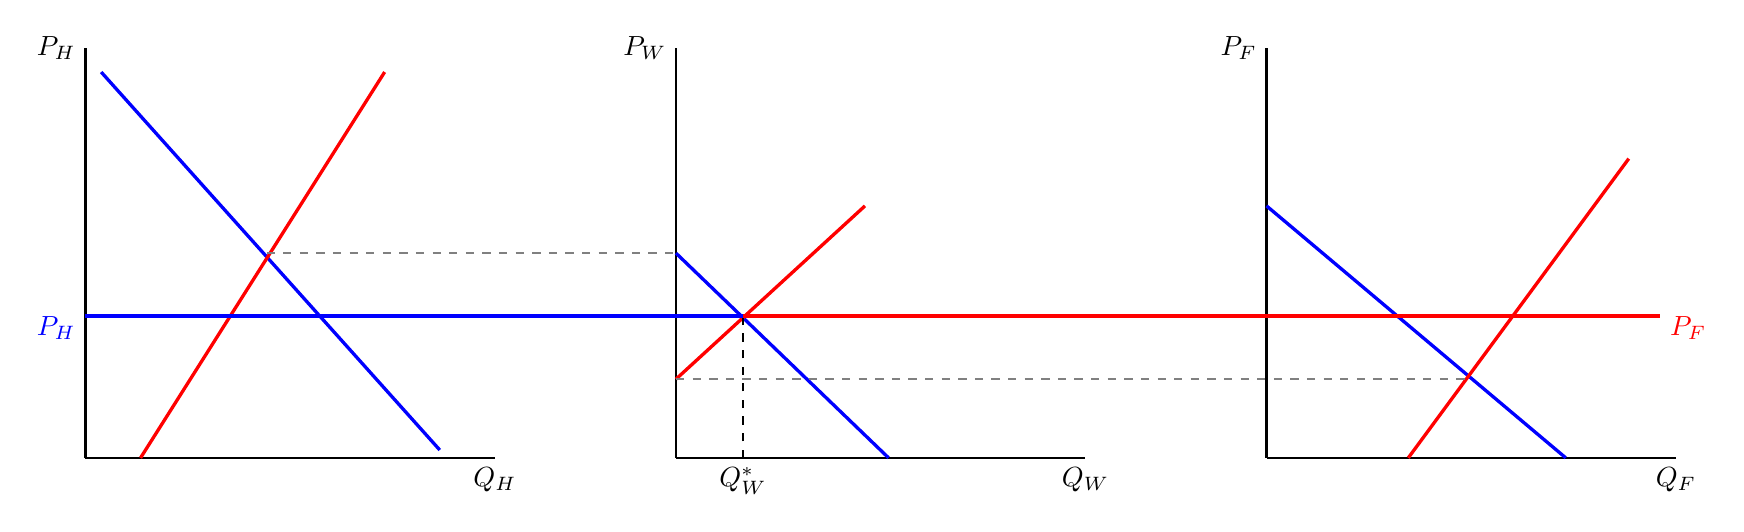
\begin{tikzpicture}[
    x=1cm,
    y=1cm,
    axis/.style={black, thick},
    demand/.style={blue, very thick},
    supply/.style={red, very thick},
    connection/.style={gray, thick, dashed}
]

% =========================================================
% PARAMETRI
% =========================================================

\def\axisheight{5.2}
\def\axiswidth{5.2}

% Posizione dei tre grafici
\def\xH{0}
\def\xW{7.5}
\def\xF{15}

% =========================================================
% MERCATO H
% =========================================================

% Assi
\draw[axis] (\xH,0) -- (\xH,\axisheight);
\draw[axis] (\xH,0) -- ++(\axiswidth,0);

% Etichette
\node[left]  at (\xH,\axisheight) {$P_H$};
\node[below] at ({\xH+\axiswidth},0) {$Q_H$};

% Domanda
\draw[demand]
({\xH+0.2},4.9) -- ({\xH+4.5},0.1);

% Offerta
\draw[supply]
({\xH+0.7},0) -- ({\xH+3.8},4.9);


% =========================================================
% MERCATO W
% =========================================================

% Assi
\draw[axis] (\xW,0) -- (\xW,\axisheight);
\draw[axis] (\xW,0) -- ++(\axiswidth,0);

% Etichette
\node[left]  at (\xW,\axisheight) {$P_W$};
\node[below] at ({\xW+\axiswidth},0) {$Q_W$};
\node[below] at ({\xW+0.85},0) {$Q^*_W$};

% Domanda
\draw[demand]
(\xW,2.6) -- ({\xW+2.7},0);

% Offerta
\draw[supply]
(\xW,1.0) -- ({\xW+2.4},3.2);

% verticale
\draw[dashed, thick] ({\xW+0.85},0) -- ({\xW+0.85},1.8);

% =========================================================
% MERCATO F
% =========================================================

% Assi
\draw[axis] (\xF,0) -- (\xF,\axisheight);
\draw[axis] (\xF,0) -- ++(\axiswidth,0);

% Etichette
\node[left]  at (\xF,\axisheight) {$P_F$};
\node[below] at ({\xF+\axiswidth},0) {$Q_F$};

% Domanda
\draw[demand]
({\xF+0.0},3.2) -- ({\xF+3.8},0);

% Offerta
\draw[supply]
({\xF+1.8},0) -- ({\xF+4.6},3.8);


% =========================================================
% LINEE CHE COLLEGANO I MERCATI
% =========================================================

% Linea superiore: H -> W
\draw[connection]
({\xH+2.3},2.6) -- (\xW,2.6);

% Linea inferiore: W -> F
\draw[connection]
(\xW,1.0) -- ({\xF+2.6},1.0);


% =========================================================
% PREZZO COMUNE H-W
% =========================================================

\draw[blue, very thick]
(\xH,1.8) -- ({\xW+0.85},1.8);

\node[blue, left]
at (\xH,1.65) {$P_H$};


% =========================================================
% PREZZO COMUNE W-F
% =========================================================

\draw[red, very thick]
({\xW+0.85},1.8) -- ({\xF+5.0},1.8);

\node[red, right]
at ({\xF+5.0},1.65) {$P_F$};

\end{tikzpicture}

}
\caption{Collegamento tra i mercati $H$, $W$ e $F$.}
\label{fig:mercati_HWF}
\end{figure}

\subsection{Politiche e loro valutazione}

\subsubsection{Introduzione di una tariffa}

Supponiamo ora che il paese $H$ voglia limitare le importazioni
introducendo una tariffa $t$ per ogni unità del bene importata da
$F$.

In assenza della tariffa, un produttore di $F$ può vendere il bene
nel proprio paese oppure in $H$ allo stesso prezzo internazionale.
Con l'introduzione della tariffa, invece, l'esportatore deve
sostenere un costo aggiuntivo pari a $t$ per ogni unità venduta
in $H$.

Immediatamente dopo l'introduzione della tariffa, esportare verso
$H$ diventa quindi meno conveniente. La riduzione degli scambi
produce due effetti.

Nel paese $H$ si genera un eccesso di domanda e il prezzo tende
ad aumentare. Nel paese $F$ si genera invece un eccesso di offerta
e il prezzo tende a diminuire.

Il processo continua fino a quando la differenza tra i prezzi nei
due paesi è esattamente pari alla tariffa:

\begin{equation*}
    P_H=P_F+t.
    \label{eq:tariffa-prezzi}
\end{equation*}

La tariffa crea quindi un divario tra i prezzi nazionali e riduce
la quantità scambiata rispetto all'equilibrio di libero commercio.


\subsubsection{Introduzione di un sussidio alle esportazioni}

Consideriamo ora una politica differente. Supponiamo che il paese
$F$ eroghi ai propri produttori un sussidio $t$ per ogni unità
esportata verso $H$.

Il sussidio aumenta la convenienza a vendere nel mercato estero.
Le imprese di $F$ cercano quindi di aumentare le esportazioni verso
$H$.

Nel paese $F$ si genera una pressione al rialzo sul prezzo interno,
mentre in $H$ la maggiore disponibilità di beni importati esercita
una pressione al ribasso sul prezzo.

Il processo continua fino a quando

\begin{equation*}
    P_F=P_H+t.
    \label{eq:sussidio-prezzi}
\end{equation*}

A differenza della tariffa, il sussidio determina quindi una
quantità scambiata superiore a quella che si avrebbe in assenza
dell'intervento.


\subsubsection{Dal modello economico a una procedura di calcolo}

Possiamo ora tradurre il ragionamento economico in una sequenza
ordinata di operazioni.

Date le curve di domanda e offerta dei due paesi, la procedura
consiste innanzitutto nel costruire le curve di domanda e offerta
sul mercato internazionale e nel determinarne l'equilibrio.

Indichiamo con $Q_{\mathrm{ex}}$ la quantità che viene effettivamente
scambiata dopo l'intervento. Nel caso di una tariffa scegliamo una
quantità inferiore alla quantità di libero scambio:

\begin{equation*}
    Q_{\mathrm{ex}}<Q_W^*,
\end{equation*}

mentre nel caso di un sussidio consideriamo

\begin{equation*}
    Q_{\mathrm{ex}}>Q_W^*.
\end{equation*}

Una volta determinata $Q_{\mathrm{ex}}$, il prezzo nel paese $H$
può essere ricavato dalla curva di domanda internazionale, mentre
il prezzo nel paese $F$ può essere ricavato dalla curva di offerta
internazionale.

La differenza tra i due prezzi determina l'ammontare della tariffa
o del sussidio:

\begin{equation*}
    \mathrm{priceGap}
    =
    \left|P_H-P_F\right|.
    \label{eq:price-gap}
\end{equation*}

Abbiamo così trasformato il modello teorico in una vera e propria
\emph{procedura di calcolo}: a partire da determinati dati di input,
eseguiamo una sequenza di operazioni per ottenere gli output di
interesse.


\begin{figure}[ht]
\centering
\resizebox{\linewidth}{!}{%
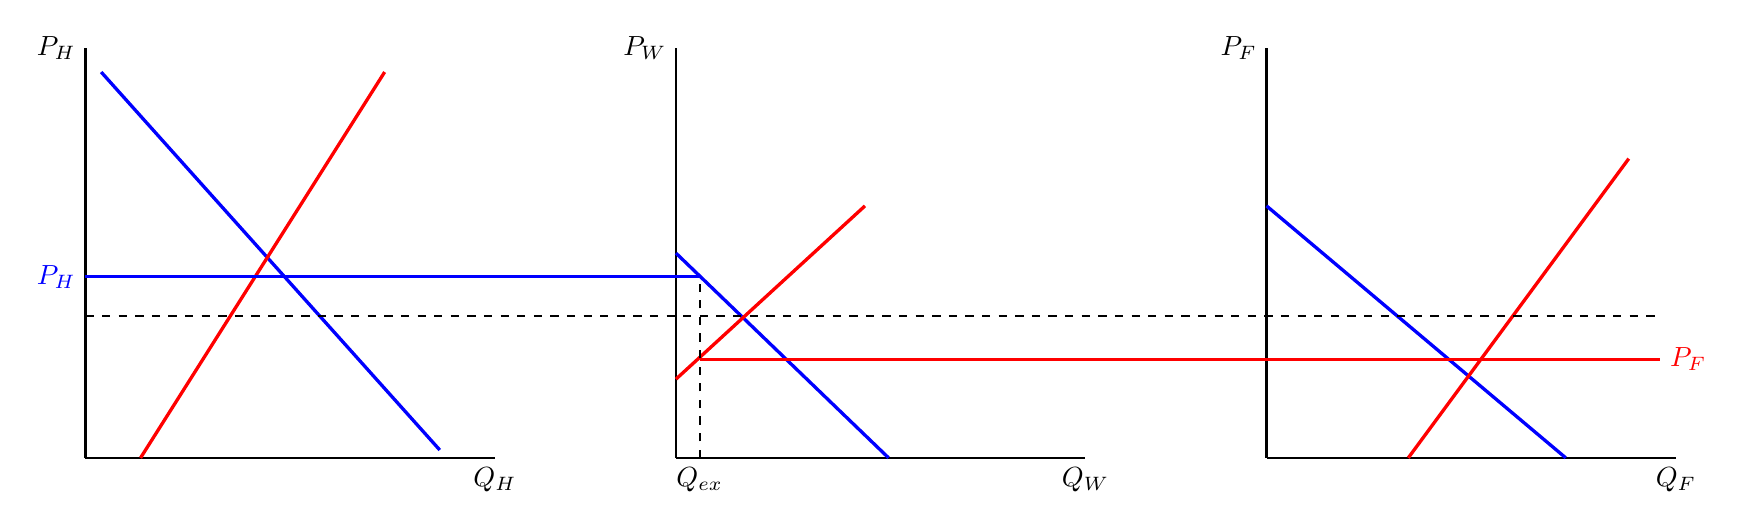
\begin{tikzpicture}[
    x=1cm,
    y=1cm,
    axis/.style={black, thick},
    demand/.style={blue, very thick},
    supply/.style={red, very thick},
    connection/.style={gray, thick, dashed}
]

% =========================================================
% PARAMETRI
% =========================================================

\def\axisheight{5.2}
\def\axiswidth{5.2}

% Posizione dei tre grafici
\def\xH{0}
\def\xW{7.5}
\def\xF{15}

% =========================================================
% MERCATO H
% =========================================================

% Assi
\draw[axis] (\xH,0) -- (\xH,\axisheight);
\draw[axis] (\xH,0) -- ++(\axiswidth,0);

% Etichette
\node[left]  at (\xH,\axisheight) {$P_H$};
\node[below] at ({\xH+\axiswidth},0) {$Q_H$};

% Domanda
\draw[demand]
({\xH+0.2},4.9) -- ({\xH+4.5},0.1);

% Offerta
\draw[supply]
({\xH+0.7},0) -- ({\xH+3.8},4.9);


% =========================================================
% MERCATO W
% =========================================================

% Assi
\draw[axis] (\xW,0) -- (\xW,\axisheight);
\draw[axis] (\xW,0) -- ++(\axiswidth,0);

% Etichette
\node[left]  at (\xW,\axisheight) {$P_W$};
\node[below] at ({\xW+\axiswidth},0) {$Q_W$};
\node[below] at ({\xW+0.3},0) {$Q_{ex}$};

% Domanda
\draw[demand]
(\xW,2.6) -- ({\xW+2.7},0);

% Offerta
\draw[supply]
(\xW,1.0) -- ({\xW+2.4},3.2);

% verticale
\draw[dashed, thick] ({\xW+0.3},0) -- ({\xW+0.3},2.3);

% =========================================================
% MERCATO F
% =========================================================

% Assi
\draw[axis] (\xF,0) -- (\xF,\axisheight);
\draw[axis] (\xF,0) -- ++(\axiswidth,0);

% Etichette
\node[left]  at (\xF,\axisheight) {$P_F$};
\node[below] at ({\xF+\axiswidth},0) {$Q_F$};

% Domanda
\draw[demand]
({\xF+0.0},3.2) -- ({\xF+3.8},0);

% Offerta
\draw[supply]
({\xF+1.8},0) -- ({\xF+4.6},3.8);


% =========================================================
% LINEE CHE COLLEGANO I MERCATI
% =========================================================

% Linea superiore: H -> W
%\draw[connection]
%({\xH+2.3},2.6) -- (\xW,2.6);

% Linea inferiore: W -> F
%\draw[connection]
%(\xW,1.0) -- ({\xF+2.6},1.0);

\draw[dashed, thick]
(\xH,1.8) -- ({\xF+5.0},1.8);

% =========================================================
% PREZZO COMUNE H-W
% =========================================================

\draw[blue, very thick]
(\xH,2.3) -- ({\xW+0.3},2.3);

\node[blue, left]
at (\xH,2.3) {$P_H$};


% =========================================================
% PREZZO COMUNE W-F
% =========================================================

\draw[red, very thick]
({\xW+0.3},1.25) -- ({\xF+5.0},1.25);

\node[red, right]
at ({\xF+5.0},1.25) {$P_F$};

\end{tikzpicture}

}
\caption{Effetti dell'introduzione di una tariffa nel paese $H$ per ridurre le importazioni.}
\label{fig:mercati_HWF_tariffa}
\end{figure}

\begin{figure}[ht]
\centering
\resizebox{\linewidth}{!}{%
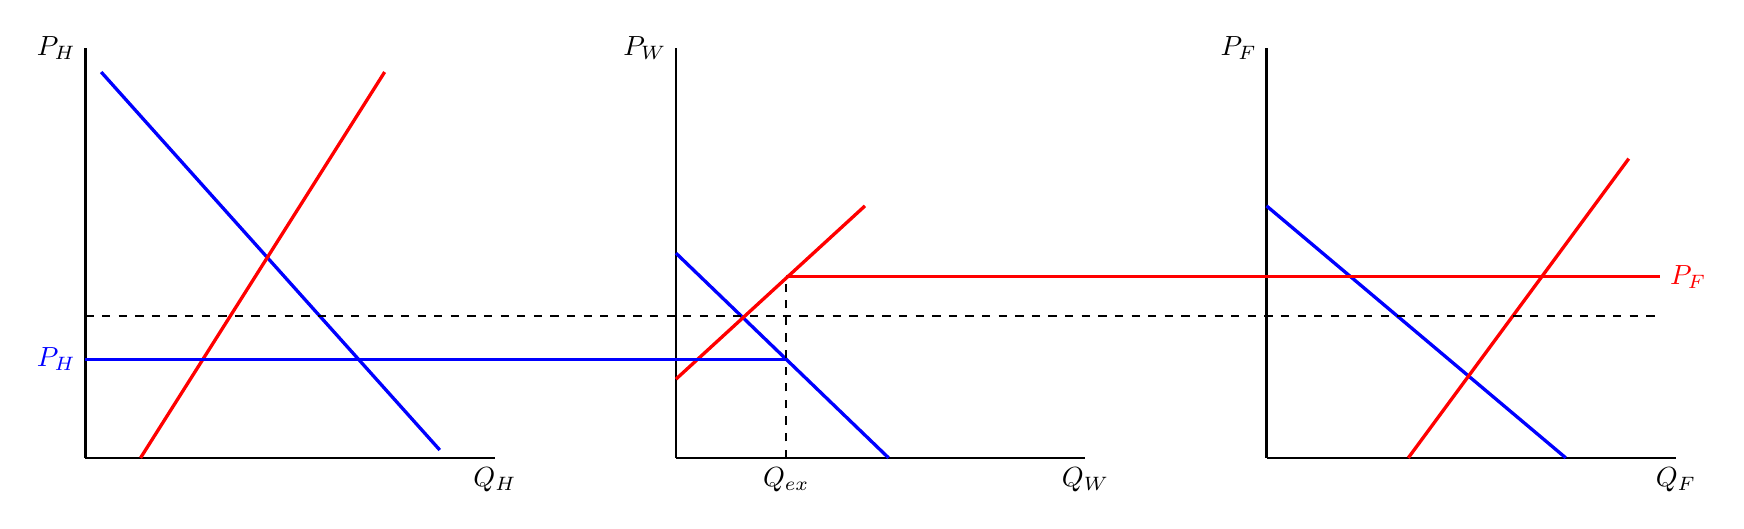
\begin{tikzpicture}[
    x=1cm,
    y=1cm,
    axis/.style={black, thick},
    demand/.style={blue, very thick},
    supply/.style={red, very thick},
    connection/.style={gray, thick, dashed}
]

% =========================================================
% PARAMETRI
% =========================================================

\def\axisheight{5.2}
\def\axiswidth{5.2}

% Posizione dei tre grafici
\def\xH{0}
\def\xW{7.5}
\def\xF{15}

% =========================================================
% MERCATO H
% =========================================================

% Assi
\draw[axis] (\xH,0) -- (\xH,\axisheight);
\draw[axis] (\xH,0) -- ++(\axiswidth,0);

% Etichette
\node[left]  at (\xH,\axisheight) {$P_H$};
\node[below] at ({\xH+\axiswidth},0) {$Q_H$};

% Domanda
\draw[demand]
({\xH+0.2},4.9) -- ({\xH+4.5},0.1);

% Offerta
\draw[supply]
({\xH+0.7},0) -- ({\xH+3.8},4.9);


% =========================================================
% MERCATO W
% =========================================================

% Assi
\draw[axis] (\xW,0) -- (\xW,\axisheight);
\draw[axis] (\xW,0) -- ++(\axiswidth,0);

% Etichette
\node[left]  at (\xW,\axisheight) {$P_W$};
\node[below] at ({\xW+\axiswidth},0) {$Q_W$};
\node[below] at ({\xW+1.4},0) {$Q_{ex}$};

% Domanda
\draw[demand]
(\xW,2.6) -- ({\xW+2.7},0);

% Offerta
\draw[supply]
(\xW,1.0) -- ({\xW+2.4},3.2);

% verticale
\draw[dashed, thick] ({\xW+1.4},0) -- ({\xW+1.4},2.3);

% =========================================================
% MERCATO F
% =========================================================

% Assi
\draw[axis] (\xF,0) -- (\xF,\axisheight);
\draw[axis] (\xF,0) -- ++(\axiswidth,0);

% Etichette
\node[left]  at (\xF,\axisheight) {$P_F$};
\node[below] at ({\xF+\axiswidth},0) {$Q_F$};

% Domanda
\draw[demand]
({\xF+0.0},3.2) -- ({\xF+3.8},0);

% Offerta
\draw[supply]
({\xF+1.8},0) -- ({\xF+4.6},3.8);


% =========================================================
% LINEE CHE COLLEGANO I MERCATI
% =========================================================

% Linea superiore: H -> W
%\draw[connection]
%({\xH+2.3},2.6) -- (\xW,2.6);

% Linea inferiore: W -> F
%\draw[connection]
%(\xW,1.0) -- ({\xF+2.6},1.0);

\draw[dashed, thick]
(\xH,1.8) -- ({\xF+5.0},1.8);

% =========================================================
% PREZZO COMUNE H-W
% =========================================================

\draw[blue, very thick]
(\xH,1.25) -- ({\xW+1.4},1.25);

\node[blue, left]
at (\xH,1.25) {$P_H$};


% =========================================================
% PREZZO COMUNE W-F
% =========================================================

\draw[red, very thick]
({\xW+1.4},2.3) -- ({\xF+5.0},2.3);

\node[red, right]
at ({\xF+5.0},2.3) {$P_F$};

\end{tikzpicture}

}
\caption{Effetti dell'introduzione di un sussidio nel paese $F$ per aumentare le esportazioni.}
\label{fig:mercati_HWF_sussidio}
\end{figure}

\subsubsection{Valutazione degli effetti sul benessere}

Conoscere i nuovi prezzi e le quantità scambiate permette di
studiare gli effetti delle politiche commerciali sul benessere
dei due paesi.

Come nel modello di un singolo mercato, consideriamo il surplus
dei consumatori e quello dei produttori. In questo caso dobbiamo
però calcolarli separatamente per $H$ e per $F$, utilizzando i
rispettivi prezzi nazionali.


\subsubsection{Surplus dei consumatori}

Consideriamo genericamente uno dei due paesi e indichiamo con
$P_{\mathrm{naz}}$ il prezzo nazionale.

Utilizzando la curva di domanda

\begin{equation*}
    Q_d=\bar Q_d-aP,
\end{equation*}

determiniamo innanzitutto la quantità domandata al prezzo
$P_{\mathrm{naz}}$:

\begin{equation*}
    Q_{d,\mathrm{naz}}
    =
    \bar Q_d-aP_{\mathrm{naz}}.
\end{equation*}

Indicando con $P_{\max}$ l'intercetta della curva di domanda
sull'asse dei prezzi, il surplus dei consumatori è

\begin{equation*}
    CS
    =
    \frac{
        Q_{d,\mathrm{naz}}
        \left(P_{\max}-P_{\mathrm{naz}}\right)
    }{2}.
    \label{eq:consumer-surplus-internazionale}
\end{equation*}


\subsubsection{Surplus dei produttori}

Utilizzando la curva di offerta

\begin{equation*}
    Q_s=\bar Q_s+bP,
\end{equation*}

calcoliamo la quantità offerta al prezzo nazionale:

\begin{equation*}
    Q_{s,\mathrm{naz}}
    =
    \bar Q_s+bP_{\mathrm{naz}}.
\end{equation*}

Quando $\bar Q_s>0$, il surplus dei produttori può essere
calcolato come

\begin{equation*}
    PS
    =
    \bar Q_s P_{\mathrm{naz}}
    +
    \frac{
        \left(Q_{s,\mathrm{naz}}-\bar Q_s\right)
        P_{\mathrm{naz}}
    }{2}.
    \label{eq:producer-surplus-positive-intercept}
\end{equation*}

Se invece l'intercetta quantitativa dell'offerta non è positiva,
possiamo individuare l'intercetta della curva di offerta sull'asse
dei prezzi, $P_{\min}$, e calcolare

\begin{equation*}
    PS
    =
    \frac{
        Q_{s,\mathrm{naz}}
        \left(P_{\mathrm{naz}}-P_{\min}\right)
    }{2}.
    \label{eq:producer-surplus-negative-intercept}
\end{equation*}


\subsubsection{Il surplus del governo}

L'introduzione di una tariffa o di un sussidio coinvolge anche il
governo.

Nel caso della tariffa, il governo di $H$ riceve un gettito pari
alla tariffa unitaria moltiplicata per la quantità importata:

\begin{equation*}
    GS_H
    =
    \mathrm{priceGap}\,Q_{\mathrm{ex}},
\end{equation*}

mentre

\begin{equation*}
    GS_F=0.
\end{equation*}

Nel caso del sussidio, il governo di $F$ sostiene invece una spesa.
Possiamo rappresentarla come un surplus negativo:

\begin{equation*}
    GS_F
    =
    -\mathrm{priceGap}\,Q_{\mathrm{ex}},
\end{equation*}

mentre

\begin{equation*}
    GS_H=0.
\end{equation*}

Per ciascun paese il surplus totale è quindi dato dalla somma di
surplus dei consumatori, surplus dei produttori e surplus del
governo:

\begin{equation*}
    TS=CS+PS+GS.
    \label{eq:total-surplus-trade}
\end{equation*}


\subsubsection{Confrontare scenari alternativi}

Per valutare l'effetto di una politica commerciale non è sufficiente
calcolare il surplus dopo l'intervento. È necessario confrontarlo
con una situazione di riferimento.

Nel caso di una tariffa, ad esempio, dobbiamo calcolare per ciascun
paese il surplus totale prima e dopo la sua introduzione.

Per il paese $H$ avremo

\begin{equation*}
    \Delta TS_H
    =
    TS_H^{\mathrm{dopo}}
    -
    TS_H^{\mathrm{prima}},
\end{equation*}

mentre per il paese $F$

\begin{equation*}
    \Delta TS_F
    =
    TS_F^{\mathrm{dopo}}
    -
    TS_F^{\mathrm{prima}}.
\end{equation*}

Il confronto tra questi valori permette di valutare come
l'intervento modifica il benessere nei due paesi.

Questo esempio evidenzia una caratteristica tipica dell'analisi
computazionale. Una stessa procedura, come il calcolo dei surplus,
deve essere eseguita ripetutamente: per paesi diversi, per prezzi
diversi e per scenari diversi.

Riscrivere ogni volta le stesse operazioni sarebbe inefficiente
e aumenterebbe la possibilità di commettere errori. È quindi utile
organizzare la procedura di calcolo in modo che possa essere
riutilizzata.


\subsection{\textbf{\textit{Strumenti di programmazione}}: le funzioni}

Una \emph{funzione} permette di raccogliere una sequenza di
operazioni che deve essere eseguita più volte.

Una funzione riceve uno o più valori di \emph{input}, li elabora
attraverso una procedura definita dall'utente e restituisce uno o
più valori di \emph{output}.

Nel nostro caso, una procedura generale per il calcolo dei surplus
può ricevere come input:

\begin{itemize}
    \item il prezzo del bene;
    \item i parametri della curva di domanda;
    \item i parametri della curva di offerta.
\end{itemize}

Utilizzando questi valori, la funzione calcola le quantità domandate
e offerte e restituisce come output il surplus dei consumatori e il
surplus dei produttori.

In forma schematica possiamo quindi rappresentare la funzione come

\begin{equation*}
\boxed{
\text{input}
\longrightarrow
\text{procedura di calcolo}
\longrightarrow
\text{output}
}
\end{equation*}

In \textsf{R}, la struttura generale di una funzione definita
dall'utente è

\begin{verbatim}
nomeFunzione <- function(input1, input2, ...) {

    # operazioni sugli input

    return(output)
}
\end{verbatim}

Una volta definita, la stessa funzione può essere richiamata
assegnando valori differenti agli input:

\begin{verbatim}
output <- nomeFunzione(valore1, valore2, ...)
\end{verbatim}

Il vantaggio non consiste soltanto nel ridurre la quantità di
codice. La funzione separa una procedura generale dai valori
specifici sui quali viene applicata. Possiamo quindi utilizzare
lo stesso algoritmo per analizzare paesi, prezzi e scenari
differenti senza dover riscrivere ogni volta la procedura di
calcolo.


\subsection{Dal problema economico all'algoritmo}

L'estensione del modello di domanda e offerta a due paesi permette
di mettere in evidenza una distinzione importante.

Il \emph{modello economico} specifica le relazioni tra domanda,
offerta, prezzi e quantità e descrive le condizioni che
caratterizzano l'equilibrio. L'\emph{algoritmo} specifica invece
la sequenza di operazioni attraverso la quale, a partire dai
parametri del modello, il computer determina i risultati.

Nel problema considerato in questa sezione possiamo sintetizzare
il procedimento come

\begin{equation*}
\boxed{
\begin{array}{c}
\text{domanda e offerta nazionali}\\
\downarrow\\
\text{prezzi di autarchia}\\
\downarrow\\
\text{domanda di importazioni e offerta di esportazioni}\\
\downarrow\\
\text{equilibrio internazionale}\\
\downarrow\\
\text{tariffa o sussidio}\\
\downarrow\\
\text{nuovi prezzi e quantità}\\
\downarrow\\
\text{surplus e variazione del benessere}
\end{array}}
\end{equation*}

Il problema economico è quindi tradotto in una successione
ordinata di operazioni che possono essere implementate in un
programma. Questa traduzione dal modello all'algoritmo costituisce
uno degli elementi centrali dell'economia computazionale.

\section{\textbf{Il modello IS--LM e la fattorizzazione LU}}
\label{sec:islm-lu}

Nelle sezioni precedenti abbiamo visto come un problema economico
possa essere rappresentato mediante un sistema di equazioni lineari

\begin{equation*}
    Ax=b.
\end{equation*}

Abbiamo inoltre introdotto l'eliminazione gaussiana, che permette
di trasformare il sistema originario in un sistema equivalente
caratterizzato da una matrice triangolare. La struttura triangolare
è particolarmente utile perché consente di determinare le incognite
in modo sequenziale.

Consideriamo ora un modello economico più articolato. Il modello
IS--LM in economia chiusa contiene più variabili endogene e ci
permette di mostrare come la soluzione di un sistema lineare possa
essere organizzata attraverso la \emph{fattorizzazione LU}.


\subsection{Il modello IS--LM}

Consideriamo il seguente modello:

\begin{align}
    Y &= C + I + \hat{G},
    \label{eq:islm-reddito}\\
    C &= \bar{C} + c(Y-\hat{T}),
    \label{eq:islm-consumo}\\
    I &= \bar{I} - bR,
    \label{eq:islm-investimento}\\
    \frac{\hat{M}}{\bar{P}} &= kY-hR.
    \label{eq:islm-moneta}
\end{align}

Le variabili endogene sono

\begin{equation*}
    Y,\qquad C,\qquad I,\qquad R,
\end{equation*}

dove $Y$ rappresenta il reddito, $C$ il consumo, $I$
l'investimento e $R$ il tasso di interesse.

Il modello contiene inoltre alcune variabili esogene. Seguendo la
distinzione adottata nel modello, $\bar C$, $\bar I$ e $\bar P$
sono considerate variabili esogene non controllabili, mentre

\begin{equation*}
    \hat G,\qquad \hat T,\qquad \hat M
\end{equation*}

sono variabili esogene controllabili dalle autorità.

Infine,

\begin{equation*}
    c,\qquad b,\qquad k,\qquad h
\end{equation*}

sono i parametri del modello.

Le quattro equazioni descrivono simultaneamente il funzionamento
del mercato dei beni e del mercato della moneta. Il problema
consiste nel determinare i valori di $Y$, $C$, $I$ e $R$ che
soddisfano contemporaneamente tutte le relazioni del modello.


\subsubsection{Dal modello economico al sistema lineare}

Per utilizzare gli strumenti numerici introdotti in precedenza,
riorganizziamo le equazioni portando le variabili endogene a
sinistra e i termini esogeni a destra.

Dall'equazione del reddito otteniamo

\begin{equation*}
    Y-C-I=\hat G.
\end{equation*}

Dalla funzione del consumo,

\begin{equation*}
    C=\bar C+c(Y-\hat T),
\end{equation*}

otteniamo

\begin{equation*}
    -cY+C=\bar C-c\hat T.
\end{equation*}

La funzione degli investimenti può essere scritta come

\begin{equation*}
    I+bR=\bar I.
\end{equation*}

Infine, l'equilibrio sul mercato monetario è

\begin{equation*}
    kY-hR=\frac{\hat M}{\bar P}.
\end{equation*}

Ordinando in ogni equazione le variabili secondo la sequenza
$Y,C,I,R$, il sistema diventa

\begin{align}
    Y-C-I+0R
        &=\hat G,\\
    -cY+C+0I+0R
        &=\bar C-c\hat T,\\
    0Y+0C+I+bR
        &=\bar I,\\
    kY+0C+0I-hR
        &=\frac{\hat M}{\bar P}.
\end{align}

Possiamo quindi scrivere il modello in forma matriciale:

\begin{equation*}
    Ax=b,
    \label{eq:islm-matrix}
\end{equation*}

dove

\begin{equation*}
A=
\begin{pmatrix}
    1  & -1 & -1 & 0\\
    -c & 1  & 0  & 0\\
    0  & 0  & 1  & b\\
    k  & 0  & 0  & -h
\end{pmatrix},
\end{equation*}

\begin{equation*}
x=
\begin{pmatrix}
    Y\\
    C\\
    I\\
    R
\end{pmatrix},
\end{equation*}

e

\begin{equation*}
b=
\begin{pmatrix}
    \hat G\\
    \bar C-c\hat T\\
    \bar I\\
    \dfrac{\hat M}{\bar P}
\end{pmatrix}.
\end{equation*}

Il problema economico è stato quindi ricondotto ancora una volta
alla soluzione di un sistema lineare. Rispetto al semplice modello
di domanda e offerta, il numero delle variabili è aumentato, ma la
struttura matematica del problema rimane la stessa.


\subsection{La fattorizzazione LU}

Una delle tecniche utilizzate per risolvere un sistema lineare con
matrice quadrata consiste nel fattorizzare la matrice $A$ come
prodotto di due matrici triangolari:

\begin{equation*}
    A=LU,
    \label{eq:lu-factorization}
\end{equation*}

dove $L$ è una matrice triangolare inferiore
(\emph{lower triangular}) e $U$ è una matrice triangolare superiore
(\emph{upper triangular}).

La fattorizzazione LU è strettamente collegata all'idea incontrata
nell'eliminazione gaussiana. Anche in questo caso, infatti,
sfruttiamo il fatto che i sistemi caratterizzati da matrici
triangolari sono particolarmente semplici da risolvere.

La differenza è che ora la trasformazione viene rappresentata
esplicitamente attraverso la decomposizione della matrice $A$ nelle
due componenti $L$ e $U$.


\subsubsection{Come la fattorizzazione LU permette di risolvere il sistema}

Partiamo dal sistema

\begin{equation*}
    Ax=b.
\end{equation*}

Poiché $A=LU$, possiamo sostituire la fattorizzazione ottenendo

\begin{equation*}
    LUx=b.
\end{equation*}

Definiamo ora un vettore ausiliario

\begin{equation*}
    y=Ux.
\end{equation*}

Il problema può essere risolto attraverso due sistemi triangolari.

Nel primo passaggio risolviamo

\begin{equation*}
    Ly=b.
    \label{eq:forward-substitution}
\end{equation*}

Poiché $L$ è triangolare inferiore, il vettore $y$ può essere
determinato mediante \emph{sostituzione in avanti}.

Una volta noto $y$, risolviamo

\begin{equation*}
    Ux=y.
    \label{eq:back-substitution}
\end{equation*}

Poiché $U$ è triangolare superiore, possiamo determinare $x$
mediante \emph{sostituzione all'indietro}.

La procedura può quindi essere sintetizzata come

\begin{equation*}
Ax=b
\quad\Longrightarrow\quad
LUx=b
\quad\Longrightarrow\quad
\begin{cases}
Ly=b,\\
Ux=y.
\end{cases}
\end{equation*}

Il problema originario viene così sostituito da due problemi
triangolari, che possono essere risolti in modo sequenziale.


\subsubsection{Esistenza della fattorizzazione LU}

La non singolarità della matrice $A$ non è, da sola, sufficiente
a garantire l'esistenza di una fattorizzazione LU nella forma
considerata.

Data una matrice

\begin{equation*}
    A\in\mathbb{R}^{n\times n},
\end{equation*}

la fattorizzazione LU esiste ed è unica se e solo se le
sottomatrici principali di ordine

\begin{equation*}
    i=1,\ldots,n-1
\end{equation*}

sono non singolari.

Le sottomatrici principali sono ottenute considerando
progressivamente le prime $i$ righe e le prime $i$ colonne della
matrice $A$.

Esistono tuttavia alcune classi di matrici per le quali l'esistenza
della fattorizzazione può essere stabilita attraverso proprietà
note. Tra queste sono particolarmente importanti le matrici a
dominanza diagonale stretta e le matrici reali simmetriche definite
positive.


\subsubsection{Strumenti di matematica: due caratteristiche delle matrici}
\paragraph{Dominanza diagonale}
Una matrice $A$ è detta \emph{a dominanza diagonale per righe} se,
per ogni riga $i$,

\begin{equation*}
    |a_{ii}|
    \geq
    \sum_{j\neq i}|a_{ij}|.
    \label{eq:diagonal-dominance}
\end{equation*}

In altri termini, il valore assoluto dell'elemento sulla diagonale
deve essere almeno pari alla somma dei valori assoluti degli altri
elementi appartenenti alla stessa riga.

La dominanza diagonale è detta \emph{stretta} quando

\begin{equation*}
    |a_{ii}|
    >
    \sum_{j\neq i}|a_{ij}|.
    \label{eq:strict-diagonal-dominance}
\end{equation*}

La stessa idea può essere applicata alle colonne, ottenendo la
definizione di dominanza diagonale per colonne.


\paragraph{Matrici definite positive}

Un'altra proprietà importante di una matrice è la definitezza.

Una matrice $A$ è detta \emph{definita positiva} se

\begin{equation*}
    x^T A x>0
    \qquad
    \forall x\neq 0.
    \label{eq:positive-definite}
\end{equation*}

L'espressione $x^TAx$ restituisce uno scalare. Infatti, se
$x\in\mathbb{R}^{n}$, allora $x^T$ ha dimensione $1\times n$,
$A$ ha dimensione $n\times n$ e $x$ ha dimensione $n\times1$.
Di conseguenza,

\begin{equation*}
    x^TAx
\end{equation*}

ha dimensione $1\times1$ e il suo segno può essere valutato.

Se si richiede invece

\begin{equation*}
    x^TAx\geq0,
\end{equation*}

la matrice viene detta \emph{semidefinita positiva}.


\subsubsection{Il caso particolare della fattorizzazione di Cholesky}

Quando $A$ è una matrice reale, simmetrica e definita positiva,
è possibile utilizzare una particolare fattorizzazione:

\begin{equation*}
    A=R^TR,
    \label{eq:cholesky}
\end{equation*}

dove $R$ è una matrice triangolare superiore con elementi positivi
sulla diagonale.

Questa decomposizione prende il nome di
\emph{fattorizzazione di Cholesky}.

Rispetto alla fattorizzazione LU generale, in questo caso è
sufficiente determinare una sola matrice triangolare, poiché
l'altra è ottenuta mediante trasposizione. Questo riduce il numero
di operazioni necessarie.


\subsubsection{Come si ottengono le matrici $L$ e $U$}

Per comprendere l'idea della fattorizzazione, consideriamo per
semplicità una matrice $3\times3$.

Cerchiamo due matrici

\begin{equation*}
L=
\begin{pmatrix}
    l_{11} & 0      & 0\\
    l_{21} & l_{22} & 0\\
    l_{31} & l_{32} & l_{33}
\end{pmatrix}
\end{equation*}

e

\begin{equation*}
U=
\begin{pmatrix}
    u_{11} & u_{12} & u_{13}\\
    0      & u_{22} & u_{23}\\
    0      & 0      & u_{33}
\end{pmatrix}
\end{equation*}

tali che

\begin{equation*}
    LU=A.
\end{equation*}

Se lasciassimo liberi tutti gli elementi non nulli di $L$ e $U$,
avremmo più incognite che equazioni. Una possibile normalizzazione
consiste quindi nell'imporre che gli elementi della diagonale di
$L$ siano uguali a uno:

\begin{equation*}
L=
\begin{pmatrix}
    1      & 0 & 0\\
    l_{21} & 1 & 0\\
    l_{31} & l_{32} & 1
\end{pmatrix}.
\end{equation*}

La condizione

\begin{equation*}
    LU=A
\end{equation*}

può essere scritta come segue:
\[
\begin{pmatrix}
u_{11} &
u_{12} &
u_{13}\\
l_{21}u_{11} &
l_{21}u_{12}+u_{22} &
l_{21}u_{13}+u_{23}\\
l_{31}u_{11} &
l_{31}u_{12}+l_{32}u_{22} &
l_{31}u_{13}+l_{32}u_{23}+u_{33}
\end{pmatrix}
=
\begin{pmatrix}
a_{11} & a_{12} & a_{13}\\
a_{21} & a_{22} & a_{23}\\
a_{31} & a_{32} & a_{33}
\end{pmatrix}.
\]
uguagliando elemento per elemento, si ottiene un sistema di equazioni dalle quali è possibile rivacare gli elementi incogniti di $L$ e $U$.

Ad esempio, confrontando l'elemento nella prima riga e prima
colonna otteniamo
\begin{equation*}
    u_{11}=a_{11},
\end{equation*}
Grazie alla struttura triangolare e alla normalizzazione della
diagonale di $L$, le prime equazioni sono particolarmente semplici
da risolvere e i valori già calcolati possono essere utilizzati
nelle equazioni successive.

Se passiamo infatti al primo elemento della seconda riga abbiamo:
\[
	l_{21}u_{11}=a_{21}\qquad\text{ma,}\ u_{11}=a_{11}\qquad \text{quindi}\qquad l_{21}=a_{21}/a_{11}.
\]

\subsubsection{fattorizzazione di Cholesky} Il procedimento è lo stesso per la fattorizzazione di Cholesky. Le equazioni da risolvere si ottengono uguagliando gli elementi delle seguenti matrici:
\[
\begin{pmatrix}
r_{11}^2 &
r_{11}r_{21} &
r_{11}r_{31}\\
r_{21}r_{11} &
r_{21}^2+r_{22}^2 &
r_{21}r_{31}+r_{22}r_{32}\\
r_{31}r_{11} &
r_{31}r_{21}+r_{32}r_{22} &
r_{31}^2+r_{32}^2+r_{33}^2
\end{pmatrix}
=
\begin{pmatrix}
a_{11} & a_{12} & a_{13}\\
a_{21} & a_{22} & a_{23}\\
a_{31} & a_{32} & a_{33}
\end{pmatrix}.
\]

Anche in questo caso le prime equazioni sono particolarmente semplici
da risolvere e i valori già calcolati possono essere utilizzati
nelle equazioni successive per calcolare tutti gli elementi di $R$.

Nelle applicazioni non sarà tuttavia necessario costruire
manualmente $L$ e $U$ o $R$: utilizzeremo le procedure di
fattorizzazione disponibili nei software di calcolo scientifico.


\subsubsection{Il ruolo del pivoting}

La fattorizzazione LU nella forma appena descritta può incontrare
difficoltà quando durante il procedimento gli elementi utilizzati
come \emph{pivot} non sono adatti all'eliminazione.

In questi casi è possibile modificare l'ordine delle righe della
matrice. Il \emph{pivoting} consiste nello scambiare opportunamente
le righe scegliendo elementi più adatti come pivot.

Questa estensione consente di applicare la fattorizzazione anche
in situazioni nelle quali le condizioni precedentemente illustrate
non sono direttamente soddisfatte.

Per il momento ci limitiamo a richiamare l'esistenza di questa
tecnica, rinviando a trattazioni più approfondite per la
costruzione dettagliata dell'algoritmo.


\subsubsection{Un ulteriore vantaggio della fattorizzazione LU}

La fattorizzazione LU può essere utile anche per calcolare il
determinante di una matrice.

Ricordiamo che

\begin{equation*}
    A=LU.
\end{equation*}

Poiché il determinante del prodotto di due matrici soddisfa

\begin{equation*}
    \det(LU)=\det(L)\det(U),
\end{equation*}

abbiamo

\begin{equation*}
    \det(A)=\det(L)\det(U).
\end{equation*}

Poiché la diagonale di $L$ sia costituita interamente da
elementi uguali a uno,

\begin{equation*}
    \det(L)=1.
\end{equation*}

Inoltre, poiché $U$ è triangolare, il suo determinante è il prodotto
degli elementi della diagonale:

\begin{equation*}
    \det(U)=\prod_{i=1}^{n}u_{ii}.
\end{equation*}

Di conseguenza,

\begin{equation*}
    \det(A)=\prod_{i=1}^{n}u_{ii}.
    \label{eq:det-lu}
\end{equation*}

Una volta ottenuta la fattorizzazione LU, il determinante può quindi
essere calcolato molto agevolmente, senza ricorrere allo sviluppo
di Laplace discusso in precedenza.


\subsection{Soluzione del modello}

I principali ambienti di calcolo scientifico mettono a disposizione
funzioni specifiche per ottenere la fattorizzazione LU.

In \textsf{R}, utilizzando il pacchetto \textsf{Matrix}, possiamo
utilizzare

\begin{verbatim}
lu(A)
\end{verbatim}

In \textsf{Octave}:

\begin{verbatim}
lu(A)
\end{verbatim}

In \textsf{Python}, attraverso \textsf{SciPy}:

\begin{verbatim}
scipy.linalg.lu(A)
\end{verbatim}

mentre in \textsf{Julia} è disponibile la funzione

\begin{verbatim}
LinearAlgebra.lu(A)
\end{verbatim}

Indipendentemente dal linguaggio utilizzato, la logica
computazionale può essere sintetizzata nei seguenti passaggi:

\begin{enumerate}
    \item assegnare la matrice $A$ e il vettore $b$;
    \item ottenere la fattorizzazione di $A$ nelle matrici
          triangolari $L$ e $U$;
    \item risolvere il sistema
          \begin{equation*}
              Ly=b
          \end{equation*}
          per determinare $y$;
    \item risolvere il sistema
          \begin{equation*}
              Ux=y
          \end{equation*}
          per determinare $x$.
\end{enumerate}

Applichiamo ora al modello IS--LM, supponendo che i parametri del modello assumano i seguenti valori:
\[
c=0.63, \qquad
b=1500, \qquad
k=0.6, \qquad
h=2700.
\]
e che le variabili esogene siano fissate ai seguenti valori:
\[
\bar{C}=55, \qquad
\bar{I}=75, \qquad
\hat{G}=200, \qquad
\hat{T}=110, \qquad
\hat{M}=200, \qquad
\bar{P}=1.
\]

Utilizzando questa parametrizzazione, la matrice $A$ è il vettore $d$ sono dati da:

\[
A=
\begin{pmatrix}
1 & -1 & -1 & 0 \\
-0.63 & 1 & 0 & 0 \\
0 & 0 & 1 & 1500 \\
0.60 & 0 & 0 & -2700
\end{pmatrix}\qquad
d=
\begin{pmatrix}
200 \\
-14.3 \\
75 \\
200
\end{pmatrix}.
\]
La fattorizzazione della matrice $A$ è la seguente:
\[
L=
\begin{pmatrix}
1 & 0 & 0 & 0 \\
-0.63 & 1 & 0 & 0 \\
0 & 0 & 1 & 0 \\
0.60 & 1.621622 & 1.621622 & 1
\end{pmatrix}
\qquad
U=
\begin{pmatrix}
1 & -1 & -1 & 0 \\
0 & 0.37 & -0.63 & 0 \\
0 & 0 & 1 & 1500 \\
0 & 0 & 0 & -5132.432
\end{pmatrix}
\]
La soluzione del sistema $Ly=d$ è:
\[
y=
\begin{pmatrix}
200 \\
111.7 \\
75 \\
-222.7568
\end{pmatrix}.
\]
ed infine otteniamo la soluzione risolvendo il sistema $Ux=y$
che fornisce simultaneamente i valori di equilibrio delle quattro variabili endogene.

\begin{equation*}
x=
\begin{pmatrix}
	Y=528.64\\
	C=318.74\\
	I=9.8973\\
	R=0.0434
\end{pmatrix}
\end{equation*}


L'esempio mostra quindi ancora una volta il percorso che
caratterizza l'approccio computazionale adottato in questo corso:

\begin{equation*}
\boxed{
\begin{array}{c}
\text{problema economico}\\
\downarrow\\
\text{modello IS--LM}\\
\downarrow\\
\text{sistema }Ax=b\\
\downarrow\\
\text{fattorizzazione }A=LU\\
\downarrow\\
Ly=b,\quad Ux=y\\
\downarrow\\
\text{equilibrio economico}
\end{array}}
\end{equation*}


